
%% bare_conf.tex
%% V1.3
%% 2007/01/11
%% by Michael Shell
%% See:
%% http://www.michaelshell.org/
%% for current contact information.
%%
%% This is a skeleton file demonstrating the use of IEEEtran.cls
%% (requires IEEEtran.cls version 1.7 or later) with an IEEE conference paper.
%%
%% Support sites:
%% http://www.michaelshell.org/tex/ieeetran/
%% http://www.ctan.org/tex-archive/macros/latex/contrib/IEEEtran/
%% and
%% http://www.ieee.org/

%%*************************************************************************
%% Legal Notice:
%% This code is offered as-is without any warranty either expressed or
%% implied; without even the implied warranty of MERCHANTABILITY or
%% FITNESS FOR A PARTICULAR PURPOSE! 
%% User assumes all risk.
%% In no event shall IEEE or any contributor to this code be liable for
%% any damages or losses, including, but not limited to, incidental,
%% consequential, or any other damages, resulting from the use or misuse
%% of any information contained here.
%%
%% All comments are the opinions of their respective authors and are not
%% necessarily endorsed by the IEEE.
%%
%% This work is distributed under the LaTeX Project Public License (LPPL)
%% ( http://www.latex-project.org/ ) version 1.3, and may be freely used,
%% distributed and modified. A copy of the LPPL, version 1.3, is included
%% in the base LaTeX documentation of all distributions of LaTeX released
%% 2003/12/01 or later.
%% Retain all contribution notices and credits.
%% ** Modified files should be clearly indicated as such, including  **
%% ** renaming them and changing author support contact information. **
%%
%% File list of work: IEEEtran.cls, IEEEtran_HOWTO.pdf, bare_adv.tex,
%%                    bare_conf.tex, bare_jrnl.tex, bare_jrnl_compsoc.tex
%%*************************************************************************

% *** Authors should verify (and, if needed, correct) their LaTeX system  ***
% *** with the testflow diagnostic prior to trusting their LaTeX platform ***
% *** with production work. IEEE's font choices can trigger bugs that do  ***
% *** not appear when using other class files.                            ***
% The testflow support page is at:
% http://www.michaelshell.org/tex/testflow/



% Note that the a4paper option is mainly intended so that authors in
% countries using A4 can easily print to A4 and see how their papers will
% look in print - the typesetting of the document will not typically be
% affected with changes in paper size (but the bottom and side margins will).
% Use the testflow package mentioned above to verify correct handling of
% both paper sizes by the user's LaTeX system.
%
% Also note that the "draftcls" or "draftclsnofoot", not "draft", option
% should be used if it is desired that the figures are to be displayed in
% draft mode.
%
\documentclass[10pt, conference, compsocconf]{IEEEtran}
% Add the compsocconf option for Computer Society conferences.
%
% If IEEEtran.cls has not been installed into the LaTeX system files,
% manually specify the path to it like:
% \documentclass[conference]{../sty/IEEEtran}





% Some very useful LaTeX packages include:
% (uncomment the ones you want to load)


% *** MISC UTILITY PACKAGES ***
%
%\usepackage{ifpdf}
% Heiko Oberdiek's ifpdf.sty is very useful if you need conditional
% compilation based on whether the output is pdf or dvi.
% usage:
% \ifpdf
%   % pdf code
% \else
%   % dvi code
% \fi
% The latest version of ifpdf.sty can be obtained from:
% http://www.ctan.org/tex-archive/macros/latex/contrib/oberdiek/
% Also, note that IEEEtran.cls V1.7 and later provides a builtin
% \ifCLASSINFOpdf conditional that works the same way.
% When switching from latex to pdflatex and vice-versa, the compiler may
% have to be run twice to clear warning/error messages.






% *** CITATION PACKAGES ***
%
%\usepackage{cite}
% cite.sty was written by Donald Arseneau
% V1.6 and later of IEEEtran pre-defines the format of the cite.sty package
% cite{} output to follow that of IEEE. Loading the cite package will
% result in citation numbers being automatically sorted and properly
% "compressed/ranged". e.g., [1], [9], [2], [7], [5], [6] without using
% cite.sty will become [1], [2], [5]--[7], [9] using cite.sty. cite.sty's
% cite will automatically add leading space, if needed. Use cite.sty's
% noadjust option (cite.sty V3.8 and later) if you want to turn this off.
% cite.sty is already installed on most LaTeX systems. Be sure and use
% version 4.0 (2003-05-27) and later if using hyperref.sty. cite.sty does
% not currently provide for hyperlinked citations.
% The latest version can be obtained at:
% http://www.ctan.org/tex-archive/macros/latex/contrib/cite/
% The documentation is contained in the cite.sty file itself.






% *** GRAPHICS RELATED PACKAGES ***
%
\ifCLASSINFOpdf
  % \usepackage[pdftex]{graphicx}
  % declare the path(s) where your graphic files are
  % \graphicspath{{../pdf/}{../jpeg/}}
  % and their extensions so you won't have to specify these with
  % every instance of \includegraphics
  % \DeclareGraphicsExtensions{.pdf,.jpeg,.png}
\else
  % or other class option (dvipsone, dvipdf, if not using dvips). graphicx
  % will default to the driver specified in the system graphics.cfg if no
  % driver is specified.
  % \usepackage[dvips]{graphicx}
  % declare the path(s) where your graphic files are
  % \graphicspath{{../eps/}}
  % and their extensions so you won't have to specify these with
  % every instance of \includegraphics
  % \DeclareGraphicsExtensions{.eps}
\fi
% graphicx was written by David Carlisle and Sebastian Rahtz. It is
% required if you want graphics, photos, etc. graphicx.sty is already
% installed on most LaTeX systems. The latest version and documentation can
% be obtained at: 
% http://www.ctan.org/tex-archive/macros/latex/required/graphics/
% Another good source of documentation is "Using Imported Graphics in
% LaTeX2e" by Keith Reckdahl which can be found as epslatex.ps or
% epslatex.pdf at: http://www.ctan.org/tex-archive/info/
%
% latex, and pdflatex in dvi mode, support graphics in encapsulated
% postscript (.eps) format. pdflatex in pdf mode supports graphics
% in .pdf, .jpeg, .png and .mps (metapost) formats. Users should ensure
% that all non-photo figures use a vector format (.eps, .pdf, .mps) and
% not a bitmapped formats (.jpeg, .png). IEEE frowns on bitmapped formats
% which can result in "jaggedy"/blurry rendering of lines and letters as
% well as large increases in file sizes.
%
% You can find documentation about the pdfTeX application at:
% http://www.tug.org/applications/pdftex





% *** MATH PACKAGES ***
%
%\usepackage[cmex10]{amsmath}
% A popular package from the American Mathematical Society that provides
% many useful and powerful commands for dealing with mathematics. If using
% it, be sure to load this package with the cmex10 option to ensure that
% only type 1 fonts will utilized at all point sizes. Without this option,
% it is possible that some math symbols, particularly those within
% footnotes, will be rendered in bitmap form which will result in a
% document that can not be IEEE Xplore compliant!
%
% Also, note that the amsmath package sets \interdisplaylinepenalty to 10000
% thus preventing page breaks from occurring within multiline equations. Use:
%\interdisplaylinepenalty=2500
% after loading amsmath to restore such page breaks as IEEEtran.cls normally
% does. amsmath.sty is already installed on most LaTeX systems. The latest
% version and documentation can be obtained at:
% http://www.ctan.org/tex-archive/macros/latex/required/amslatex/math/





% *** SPECIALIZED LIST PACKAGES ***
%
%\usepackage{algorithmic}
% algorithmic.sty was written by Peter Williams and Rogerio Brito.
% This package provides an algorithmic environment fo describing algorithms.
% You can use the algorithmic environment in-text or within a figure
% environment to provide for a floating algorithm. Do NOT use the algorithm
% floating environment provided by algorithm.sty (by the same authors) or
% algorithm2e.sty (by Christophe Fiorio) as IEEE does not use dedicated
% algorithm float types and packages that provide these will not provide
% correct IEEE style captions. The latest version and documentation of
% algorithmic.sty can be obtained at:
% http://www.ctan.org/tex-archive/macros/latex/contrib/algorithms/
% There is also a support site at:
% http://algorithms.berlios.de/index.html
% Also of interest may be the (relatively newer and more customizable)
% algorithmicx.sty package by Szasz Janos:
% http://www.ctan.org/tex-archive/macros/latex/contrib/algorithmicx/




% *** ALIGNMENT PACKAGES ***
%
%\usepackage{array}
% Frank Mittelbach's and David Carlisle's array.sty patches and improves
% the standard LaTeX2e array and tabular environments to provide better
% appearance and additional user controls. As the default LaTeX2e table
% generation code is lacking to the point of almost being broken with
% respect to the quality of the end results, all users are strongly
% advised to use an enhanced (at the very least that provided by array.sty)
% set of table tools. array.sty is already installed on most systems. The
% latest version and documentation can be obtained at:
% http://www.ctan.org/tex-archive/macros/latex/required/tools/


%\usepackage{mdwmath}
%\usepackage{mdwtab}
% Also highly recommended is Mark Wooding's extremely powerful MDW tools,
% especially mdwmath.sty and mdwtab.sty which are used to format equations
% and tables, respectively. The MDWtools set is already installed on most
% LaTeX systems. The lastest version and documentation is available at:
% http://www.ctan.org/tex-archive/macros/latex/contrib/mdwtools/


% IEEEtran contains the IEEEeqnarray family of commands that can be used to
% generate multiline equations as well as matrices, tables, etc., of high
% quality.


%\usepackage{eqparbox}
% Also of notable interest is Scott Pakin's eqparbox package for creating
% (automatically sized) equal width boxes - aka "natural width parboxes".
% Available at:
% http://www.ctan.org/tex-archive/macros/latex/contrib/eqparbox/





% *** SUBFIGURE PACKAGES ***
%\usepackage[tight,footnotesize]{subfigure}
% subfigure.sty was written by Steven Douglas Cochran. This package makes it
% easy to put subfigures in your figures. e.g., "Figure 1a and 1b". For IEEE
% work, it is a good idea to load it with the tight package option to reduce
% the amount of white space around the subfigures. subfigure.sty is already
% installed on most LaTeX systems. The latest version and documentation can
% be obtained at:
% http://www.ctan.org/tex-archive/obsolete/macros/latex/contrib/subfigure/
% subfigure.sty has been superceeded by subfig.sty.



%\usepackage[caption=false]{caption}
%\usepackage[font=footnotesize]{subfig}
% subfig.sty, also written by Steven Douglas Cochran, is the modern
% replacement for subfigure.sty. However, subfig.sty requires and
% automatically loads Axel Sommerfeldt's caption.sty which will override
% IEEEtran.cls handling of captions and this will result in nonIEEE style
% figure/table captions. To prevent this problem, be sure and preload
% caption.sty with its "caption=false" package option. This is will preserve
% IEEEtran.cls handing of captions. Version 1.3 (2005/06/28) and later 
% (recommended due to many improvements over 1.2) of subfig.sty supports
% the caption=false option directly:
%\usepackage[caption=false,font=footnotesize]{subfig}
%
% The latest version and documentation can be obtained at:
% http://www.ctan.org/tex-archive/macros/latex/contrib/subfig/
% The latest version and documentation of caption.sty can be obtained at:
% http://www.ctan.org/tex-archive/macros/latex/contrib/caption/




% *** FLOAT PACKAGES ***
%
%\usepackage{fixltx2e}
% fixltx2e, the successor to the earlier fix2col.sty, was written by
% Frank Mittelbach and David Carlisle. This package corrects a few problems
% in the LaTeX2e kernel, the most notable of which is that in current
% LaTeX2e releases, the ordering of single and double column floats is not
% guaranteed to be preserved. Thus, an unpatched LaTeX2e can allow a
% single column figure to be placed prior to an earlier double column
% figure. The latest version and documentation can be found at:
% http://www.ctan.org/tex-archive/macros/latex/base/



%\usepackage{stfloats}
% stfloats.sty was written by Sigitas Tolusis. This package gives LaTeX2e
% the ability to do double column floats at the bottom of the page as well
% as the top. (e.g., "\begin{figure*}[!b]" is not normally possible in
% LaTeX2e). It also provides a command:
%\fnbelowfloat
% to enable the placement of footnotes below bottom floats (the standard
% LaTeX2e kernel puts them above bottom floats). This is an invasive package
% which rewrites many portions of the LaTeX2e float routines. It may not work
% with other packages that modify the LaTeX2e float routines. The latest
% version and documentation can be obtained at:
% http://www.ctan.org/tex-archive/macros/latex/contrib/sttools/
% Documentation is contained in the stfloats.sty comments as well as in the
% presfull.pdf file. Do not use the stfloats baselinefloat ability as IEEE
% does not allow \baselineskip to stretch. Authors submitting work to the
% IEEE should note that IEEE rarely uses double column equations and
% that authors should try to avoid such use. Do not be tempted to use the
% cuted.sty or midfloat.sty packages (also by Sigitas Tolusis) as IEEE does
% not format its papers in such ways.





% *** PDF, URL AND HYPERLINK PACKAGES ***
%
%\usepackage{url}
% url.sty was written by Donald Arseneau. It provides better support for
% handling and breaking URLs. url.sty is already installed on most LaTeX
% systems. The latest version can be obtained at:
% http://www.ctan.org/tex-archive/macros/latex/contrib/misc/
% Read the url.sty source comments for usage information. Basically,
% \url{my_url_here}.





% *** Do not adjust lengths that control margins, column widths, etc. ***
% *** Do not use packages that alter fonts (such as pslatex).         ***
% There should be no need to do such things with IEEEtran.cls V1.6 and later.
% (Unless specifically asked to do so by the journal or conference you plan
% to submit to, of course. )


% correct bad hyphenation here
\hyphenation{op-tical net-works semi-conduc-tor}

\usepackage{graphicx}
\usepackage{color}
\usepackage{txfonts}
\usepackage{multirow}
%\usepackage[]{algorithm2e}
\usepackage{algpseudocode}
\usepackage{algorithm}
\usepackage{threeparttable}
%\usepackage{bibspacing}

\begin{document}

\graphicspath{{pic/}}

%
% paper title
% can use linebreaks \\ within to get better formatting as desired
\title{Automatic Construction of Callback Model for Android Application}


% author names and affiliations
% use a multiple column layout for up to two different
% affiliations

%\author{\IEEEauthorblockN{Authors Name/s per 1st Affiliation (Author)}
%\IEEEauthorblockA{line 1 (of Affiliation): dept. name of organization\\
%line 2: Nankai University, acronyms acceptable\\
%line 3: Tianjin, China
%line 4: Email: name@xyz.com}
%\and
%\IEEEauthorblockN{Authors Name/s per 2nd Affiliation (Author)}
%\IEEEauthorblockA{line 1 (of Affiliation): dept. name of organization\\
%line 2: name of organization, acronyms acceptable\\
%line 3: City, Country\\
%line 4: Email: name@xyz.com}
%}

% conference papers do not typically use \thanks and this command
% is locked out in conference mode. If really needed, such as for
% the acknowledgment of grants, issue a \IEEEoverridecommandlockouts
% after \documentclass

% for over three affiliations, or if they all won't fit within the width
% of the page, use this alternative format:
% 
\author{\IEEEauthorblockN{Chenkai Guo\IEEEauthorrefmark{1,2},
Quanqi Ye\IEEEauthorrefmark{3},
Naipeng Dong\IEEEauthorrefmark{2}, 
Guangdong Bai\IEEEauthorrefmark{4},
Jin Song Dong\IEEEauthorrefmark{2} and
Jing Xu\IEEEauthorrefmark{1}}
\IEEEauthorblockA{\IEEEauthorrefmark{1}College of Computer and Control Engineering, Nankai University}
\IEEEauthorblockA{\IEEEauthorrefmark{3}NUS Graduate School for Integrative Sciences and Engineering, National University of Singapore}
\IEEEauthorblockA{\IEEEauthorrefmark{2}School of Computing, National University of Singapore}
\IEEEauthorblockA{\IEEEauthorrefmark{4}Singapore Institute of Technology}}





% use for special paper notices
%\IEEEspecialpapernotice{(Invited Paper)}




% make the title area
\maketitle


\begin{abstract}
The heavy use of event-callback mechanism in frameworks like Android causes challenges for static analysis. Modelling of callback mechanisms for Android applications (app for short) is becoming a major method to address such challenges. In this work, we aim to construct a generic callback-related model that supports path-sensitive analysis. We consider three unresolved challenges in the existing modelling approaches: 1) building connections between different components; 2) identifying path-sensitive conditions; 3) handling the system-driven callbacks and fine-grained lifecycle callbacks. We propose algorithms for constructing a generic path-sensitive callback model and present a prototype model constructor, AndroChecker, to validate our approach. We evaluate 20 real-world apps using AndroChecker. The evaluation result shows that our method and tool have a strong capability in modelling path conditions and inter-component invocations.

%the number of targeted execution traces would grow exponentially according to the complexity of event-callbacks. 
% we represent AndroChecker, a prototype analyser for model checking a given Android app from the perspective of callbacks. Compared to prior work of app model, AndroChecker conducts a more complete callback modelling, including life-cycle, user-driven and system-driven. Moreover, AndroChecker provides defined attributes for checking specific features of target app in practise. The evaluation of 1000 apps indicates the effectiveness of our approach. 

\end{abstract}

%\begin{IEEEkeywords}
%callback transition model; data dependency; Android; 

%\end{IEEEkeywords}


% For peer review papers, you can put extra information on the cover
% page as needed:
% \ifCLASSOPTIONpeerreview
% \begin{center} \bfseries EDICS Category: 3-BBND \end{center}
% \fi
%
% For peerreview papers, this IEEEtran command inserts a page break and
% creates the second title. It will be ignored for other modes.
\IEEEpeerreviewmaketitle

%\section{Introduction}
With the rapid development of mobile devices, interactions with such devices have already become indispensable in people's daily life. To meet users' increasing service demands on mobile devices, there has been a surge in developing mission-critical programs running on the devices, called \textit{apps}. Nowadays, despite the fact that Android apps have dominated the mobile market, there are still a large amount of apps being produced every day. Consequently, the growing number of apps also raise the quality concerns, e.g., potential bugs and security issues. How to verify the correctness and security of such apps has become a critical concern for both developers and users.

Event-driven, which is a representative feature in Android systems, is well-known as the cause of intractable issues on testing and verification. Since Android apps do not have a fixed program entry, traditional flow analysis \cite{new1976program, new1978dataflow} is hard to be directly adopted to address such issues. Due to that Android framework is complex and full of event-driven structures (e.g, listener interfaces, event callbacks, etc.), static analysis for Android normally chooses to create models of an Android app rather than directly analysing the app source code. There are two ways of app modelling in term of the modelling object: \textit{callback-directed} \cite{new2013contextual,new2015static} and \textit{data-directed} \cite{new2014flowdroid, new2015DroidSafe}. Callback-directed modelling captures event-callback sequences within the targeted app and represents them as a variation of control flow graph (\textit{CFG}); whereas data-directed modelling identifies types of information related to the analysis goal and combines this information according to the flow sequences. The former way is more versatile and is able to provide logical structure over the entire app program. However, pure callback-directed modelling can hardly provide concrete assist for analysis in practical scenarios, since most of the modelling targets, functionality testing or security verification, are closely combined with solid data input and output.
Data-directed modelling has advantages in tackling specific analysis, but has a heavy cost in constructing a generic model. 

In the current stage, neither callback-directed nor data-directed modelling is able to conduct a callback model in a generic and fine-grained manner. The reason is that Android is equipped with many complex features such as inter-process communication and vast callback SDKs (Software Development Kit). As a result, the generated model by existing works, such as \cite{new2013contextual,new2015static, new2015window}, is incomplete. In details, the incompleteness exists in three aspects. 1) Component types: only \texttt{activity} is involved in the modelling; other components like \texttt{service} and \texttt{broadcast receiver} are ignored. However, security compromises and logic bugs frequently exist in service and broadcast receiver components. 2) Callback types: only callbacks related to lifecycle and user interaction are taken into consideration. Actually, in Android, a variety of callbacks are driven by system events, like phone and location status. Although these system-driven callbacks are invoked invisibly, they are of great importance in analysing certain system status. 3) Path-insensitive: in the existing callback modelling, the generated edges only present a \textit{possible} flow from a start node to an end node, ignoring information such as how and when the flow is executed. In practice, merely offering a group of \textit{possible} paths has limited help to analysis. For example, techniques for test case generation normally need to confirm the condition ranges for specifying certain program paths. In other words, the test-cases are determined by the condition data rather than the paths themselves. Therefore, constructing a path-sensitive model benefits advanced application based on the model.    

In this work, we aim to develop a generic, event-callback related modelling approach to handle the critical condition data that impacts the direction of control flows, such that our approach has both of the advantages of callback-directed and data-directed modelling. To achieve the goal, we automatically construct a generic path-sensitive callback (\textit{GPC} for short) model for each Android app. There are three key insights underlying our approach: 1) components like service run in a parallel way with other components; 2) each of the non-lifecycle callbacks needs to register itself in their parent callbacks before execution; 3) the callback execution condition can be identified by analysing the register implementation along with possible paths. Our approach leverages above insights to fully automate the model construction via static program analysis. 

We design and implement a proof-of-concept model builder AndroChecker, which receives Android \textit{apk} files as input and outputs their corresponding \textit{GPC} models. We apply AndroChecker to 20 real-world apps. The evaluation results show that our technique is both accurate and complete. 

The main contributions of this paper can be concluded as follows: 
\begin{itemize}
\item First, we defined the \textit{GPC} model, a generic path-sensitive callback model, which facilitates the understanding, testing and statically verifying Android apps.
\item Second, we proposed an algorithm to automatically construct the \textit{GPC} model, by adopting backward data dependency analysis.
\item Third, we implemented the algorithm as a proof-of-concept model builder AndroChecker.
\item Fourth, we performed experimental evaluation on 20 real-world apps, as well as three case studies, which confirms the correctness and efficiency of our method and tool.
\end{itemize}

%Insight: 1) most of the firing of callbacks must obey specific conditions, which is relevant to not only resource file\cite{}, but also data dependency.
%2) the same callback varies under different driven.(prefix sensitive)
%3) There exists impact between intra-components.(create a novel graph)
%
%In this work, we focus on constructing a generic, deep context-sensitive, cross-components framework for callback transition analysis. We seek to solve a problem 
%
%Our approach is based on deep context reasoning

\section{Introduction}
%With the rapid development of mobile devices, interactions with such devices have already become indispensable in people's daily life. To meet users' increasing service demands on mobile devices, there has been a surge in developing mission-critical programs running on the devices, called \textit{apps}. Nowadays, despite the fact that Android apps have dominated the mobile market, there are still a large amount of apps being produced every day. Consequently, the growing number of apps also raise the quality concerns, e.g., potential bugs and security issues. How to verify the correctness and security of such apps has become a critical concern for both developers and users.

Correctness and security of Android apps has become a critical concern and thus verification is needed.
%
%Event-driven, which is a representative feature in Android systems, is well-known as the cause of intractable issues on testing and verification. 
However, traditional flow analysis \cite{new1976program, new1978dataflow} is hard to be directly adopted to Android apps, since Android apps do not have a fixed program entry. A promising way of static analysis is to create models of an Android app rather than directly analysing the app source code, due to its event-driven structures (e.g, listener interfaces, event callbacks, etc.). There are two ways of app modelling: \textit{callback-directed} \cite{new2013contextual,new2015static} and \textit{data-directed} \cite{new2014flowdroid, new2015DroidSafe}. Callback-directed modelling captures event-callback sequences within the targeted app and represents them as a variation of control flow graph (\textit{CFG}); whereas data-directed modelling identifies types of information related to the analysis goal and combines this information according to the flow sequences. The former way is more versatile and is able to provide logical structure over the entire app program. However, it can hardly provide concrete assist for analysis in practical scenarios, since most of the modelling targets, functionality testing or security verification, are closely combined with solid data input and output.
Data-directed modelling has advantages in tackling specific analysis, but has a heavy cost in constructing a generic model. 
Neither of them is able to conduct a callback model in a generic and fine-grained manner. 

%The reason is that Android is equipped with many complex features such as inter-process communication and vast callback SDKs (Software Development Kit). As a result, the generated model by existing works, such as \cite{new2013contextual,new2015static, new2015window}, is incomplete. 

In more details, prior app modelling suffers from incompleteness in three aspects. 1) Component types: only \texttt{activity} is involved in the modelling; other components like \texttt{service} and \texttt{broadcast receiver} are ignored. However, security compromises and logic bugs frequently exist in \texttt{service} and \texttt{broadcast receiver} components. 2) Callback types: only callbacks related to lifecycle and user interaction are taken into consideration. Actually, in Android, a variety of callbacks are driven by system events, like phone and location status. 
%Although these system-driven callbacks are invoked invisibly, they are of great importance in analysing certain system status. 
3) Path-insensitive: in the existing callback modelling, the generated edges only present a \textit{possible} flow from a start node to an end node, ignoring information such as how and when the flow is executed. There lacks a valid way to handle the conditions of the execution of possible flows.
 
%In practice, merely offering a group of \textit{possible} paths has limited help to analysis. For example, techniques for test case generation normally need to confirm the condition ranges for specifying certain program paths. In other words, the test-cases are determined by the condition data rather than the paths themselves.Therefore, constructing a path-sensitive model benefits advanced application based on the model.
   

In this work, we develop an approach for constructing generic path-sensitive callback (\textit{GPC} for short) model for Android apps.
%we develop a generic, event-callback related modelling approach to handle the critical condition data that impacts the direction of control flows, such that our approach has both of the advantages of callback-directed and data-directed modelling. %To achieve the goal,  
There are three key insights underlying our approach: 1) components like \texttt{service} run in a parallel way with other components; 2) each of the non-lifecycle callbacks needs to register itself in their parent callbacks before execution; 3) the callback execution condition can be identified by analysing the register implementation along with possible paths. Our approach leverages the above insights to fully automate the model construction via static program analysis. 
%
We design and implement a proof-of-concept model builder AndroChecker, which receives Android \textit{apk} files as input and outputs their corresponding \textit{GPC} models. We apply AndroChecker to $20$ real-world apps. The evaluation results show that our technique is both accurate and complete. 

%The main contributions of this paper can be concluded as follows: 
%\begin{itemize}
%\item First, we defined the \textit{GPC} model, a generic path-sensitive callback model, which facilitates the understanding, testing and statically verifying Android apps.
%\item Second, we proposed an algorithm to automatically construct the \textit{GPC} model, by adopting backward data dependency analysis.
%\item Third, we implemented the algorithm as a proof-of-concept model builder AndroChecker.
%\item Fourth, we performed experimental evaluation on 20 real-world apps, as well as three case studies, which confirms the correctness and efficiency of our method and tool.
%\end{itemize}

%Insight: 1) most of the firing of callbacks must obey specific conditions, which is relevant to not only resource file\cite{}, but also data dependency.
%2) the same callback varies under different driven.(prefix sensitive)
%3) There exists impact between intra-components.(create a novel graph)
%
%In this work, we focus on constructing a generic, deep context-sensitive, cross-components framework for callback transition analysis. We seek to solve a problem 
%
%Our approach is based on deep context reasoning

%\section{Background} \label{background}
Android is known as the domain operating system for mobile devices, which is based on Linux, middleware and vast of core libraries. Developers can develop specialized apps using the libraries offered by Android. The main program modules of Android apps are called \textit{components}. There are four types of component in Android system: activity, service, broadcast recevier and content provider. \textit{Activity} is used to handle tasks for interacting with user; while \textit{service} handles computing tasks in the background. A \textit{broadcast recevier} is used to respond to the broadcast from system or other components. A \textit{content provider} works for data management. The communication between components relies on \textit{intent}.

Typically, Android program is event-driven and lacks an explicit fixed entry point for program execution.  
Instead, the app execution is driven by certain events from either system or user. Each component within the app consists of a number of callbacks to respond to the events. Normally Android callbacks are implemented by overriding methods in relative listener interfaces. Here we divide the callbacks into three categories in terms of their usages.
 
\textbf{Lifecycle callbacks} respond to lifecycle events that reflect life stages of holder component. In the four types of component, activity supports a more complex lifecycle since it acts as a main channel for interacting with user. As a result, prior works tend to construct activity-oriented model. Yet, other components also have their own lifecycle callbacks though simpler. Specifically, service has two sets of different lifecycle callbacks, supporting binding and launching operations from other component, respectively. 

\textbf{\textit{GUI} callbacks} handle the visual interaction with user. Therefore they are normally implemented in activity. \textit{GUI} callbacks are implemented in the listener interfaces that have a common superclass \texttt{android.view.View}. These interfaces need to be registered in other callback via API like \texttt{setOnClickListener}.

\textbf{System-driven callbacks} are normally invoked when a specific system status changes. Analogous with \textit{GUI} callbacks, system-driven callbacks are held by certain Android listener interfaces. These interfaces start to listen specialized events after they are registered and end the listening when they are unregistered. Though vast of system listener interfaces are supplied in Android, they adopt similar register and unregister manners connecting the holder callbacks with corresponding system-driven callbacks. 

We call the \textit{GUI} and system-driven callbacks \textit{non-lifecycle callback} hereafter. Non-lifecycle callbacks are always invoked in specialized \textit{running interval} for each component. In activity, the running interval refers to the region between \texttt{onResume} and \texttt{onPause}. In service, the interval is located between \texttt{onStartCommand} and \texttt{onDestroy}, or \texttt{onBind} and \texttt{onUnbind}.

\textit{Callback control flow} \textit{CCF} (callback control flow)\cite{new2015static} presents underlying time sequences for each callback. For lifecycle callbacks, the flow sequences are simply along with the lifecycle sequences. However, as mentioned before, non-lifecycle callbacks have to be registered before they are invoked via events. Thus the holder callback $ \eta $ has to be invoked before the registered callback $ \zeta $. In this way, there exists a potential flow from $ \eta $ to $ \zeta $, denoted as $ \eta \rightarrow \zeta $. Actually, $ \zeta $ are not directly invoked by $ \eta $, but activated when $ \eta $ is invoked. The edge $ \rightarrow $ reflects a \textit{possible} invocation sequence between $ \eta $ and $ \zeta $. Here the \texttt{onReceive} callback of broadcast receiver is also regarded as non-lifecycle callbacks. Dynamically registered broadcast receiver acts as an event listener within the holder component (activity or service). At the same time, broadcast receiver statically registered in the \textit{Androidmanifest.xml} runs along with foreground activity. Therefore, it can be treated as the event listener of foreground activity although there is not a specified fixed holder. Note that we don't consider the content provider in this work since it is only used for data management and it lacks of useful callback implementation. 

Another flow type within the \textit{CCF} comes from the inter-components invocation where the invoker and invokee components are combined by connection site like \texttt{startActivity} and \texttt{startService}. If both of the invoker $ \eta $ and invokee $ \zeta $ belong to activity, there exists s strict time sequence $ \eta \rightarrow \zeta $. When the invokee activity starts running on the foreground, the invoker has already been moved to background and stopped running. If either the invoker or invokee involves service, the invocation will be treated as \textit{parallel edge} since service can run in parallel with other components, which is not considered in \cite{new2015static}. At this time, the sequence between the invoker and the invokee is flexible. In the inter-component cases, the \texttt{onCreate} of the launcher activity (registered as \texttt{android.intent.category.LAUNCHER} in the \textit{Androidmanifest.xml}) is treated as the entry point of entire system.
%\section{Overview}\label{overview}
We illustrate our approach using a real-world app from open-source Android distribution \textit{f-Droid}~\cite{newFDroid} as example. We first introduce the app by describing the source code snippet shown in Figure 1 (Section \ref{motivation}). Then we define the problem raised by the example app (Section \ref{problem-define}) and propose solution and algorithms addressing the problem (Section\ref{algorithms}). 
\subsection{Motivation} \label{motivation}

\begin{figure}[htbp]  
  \centering  
  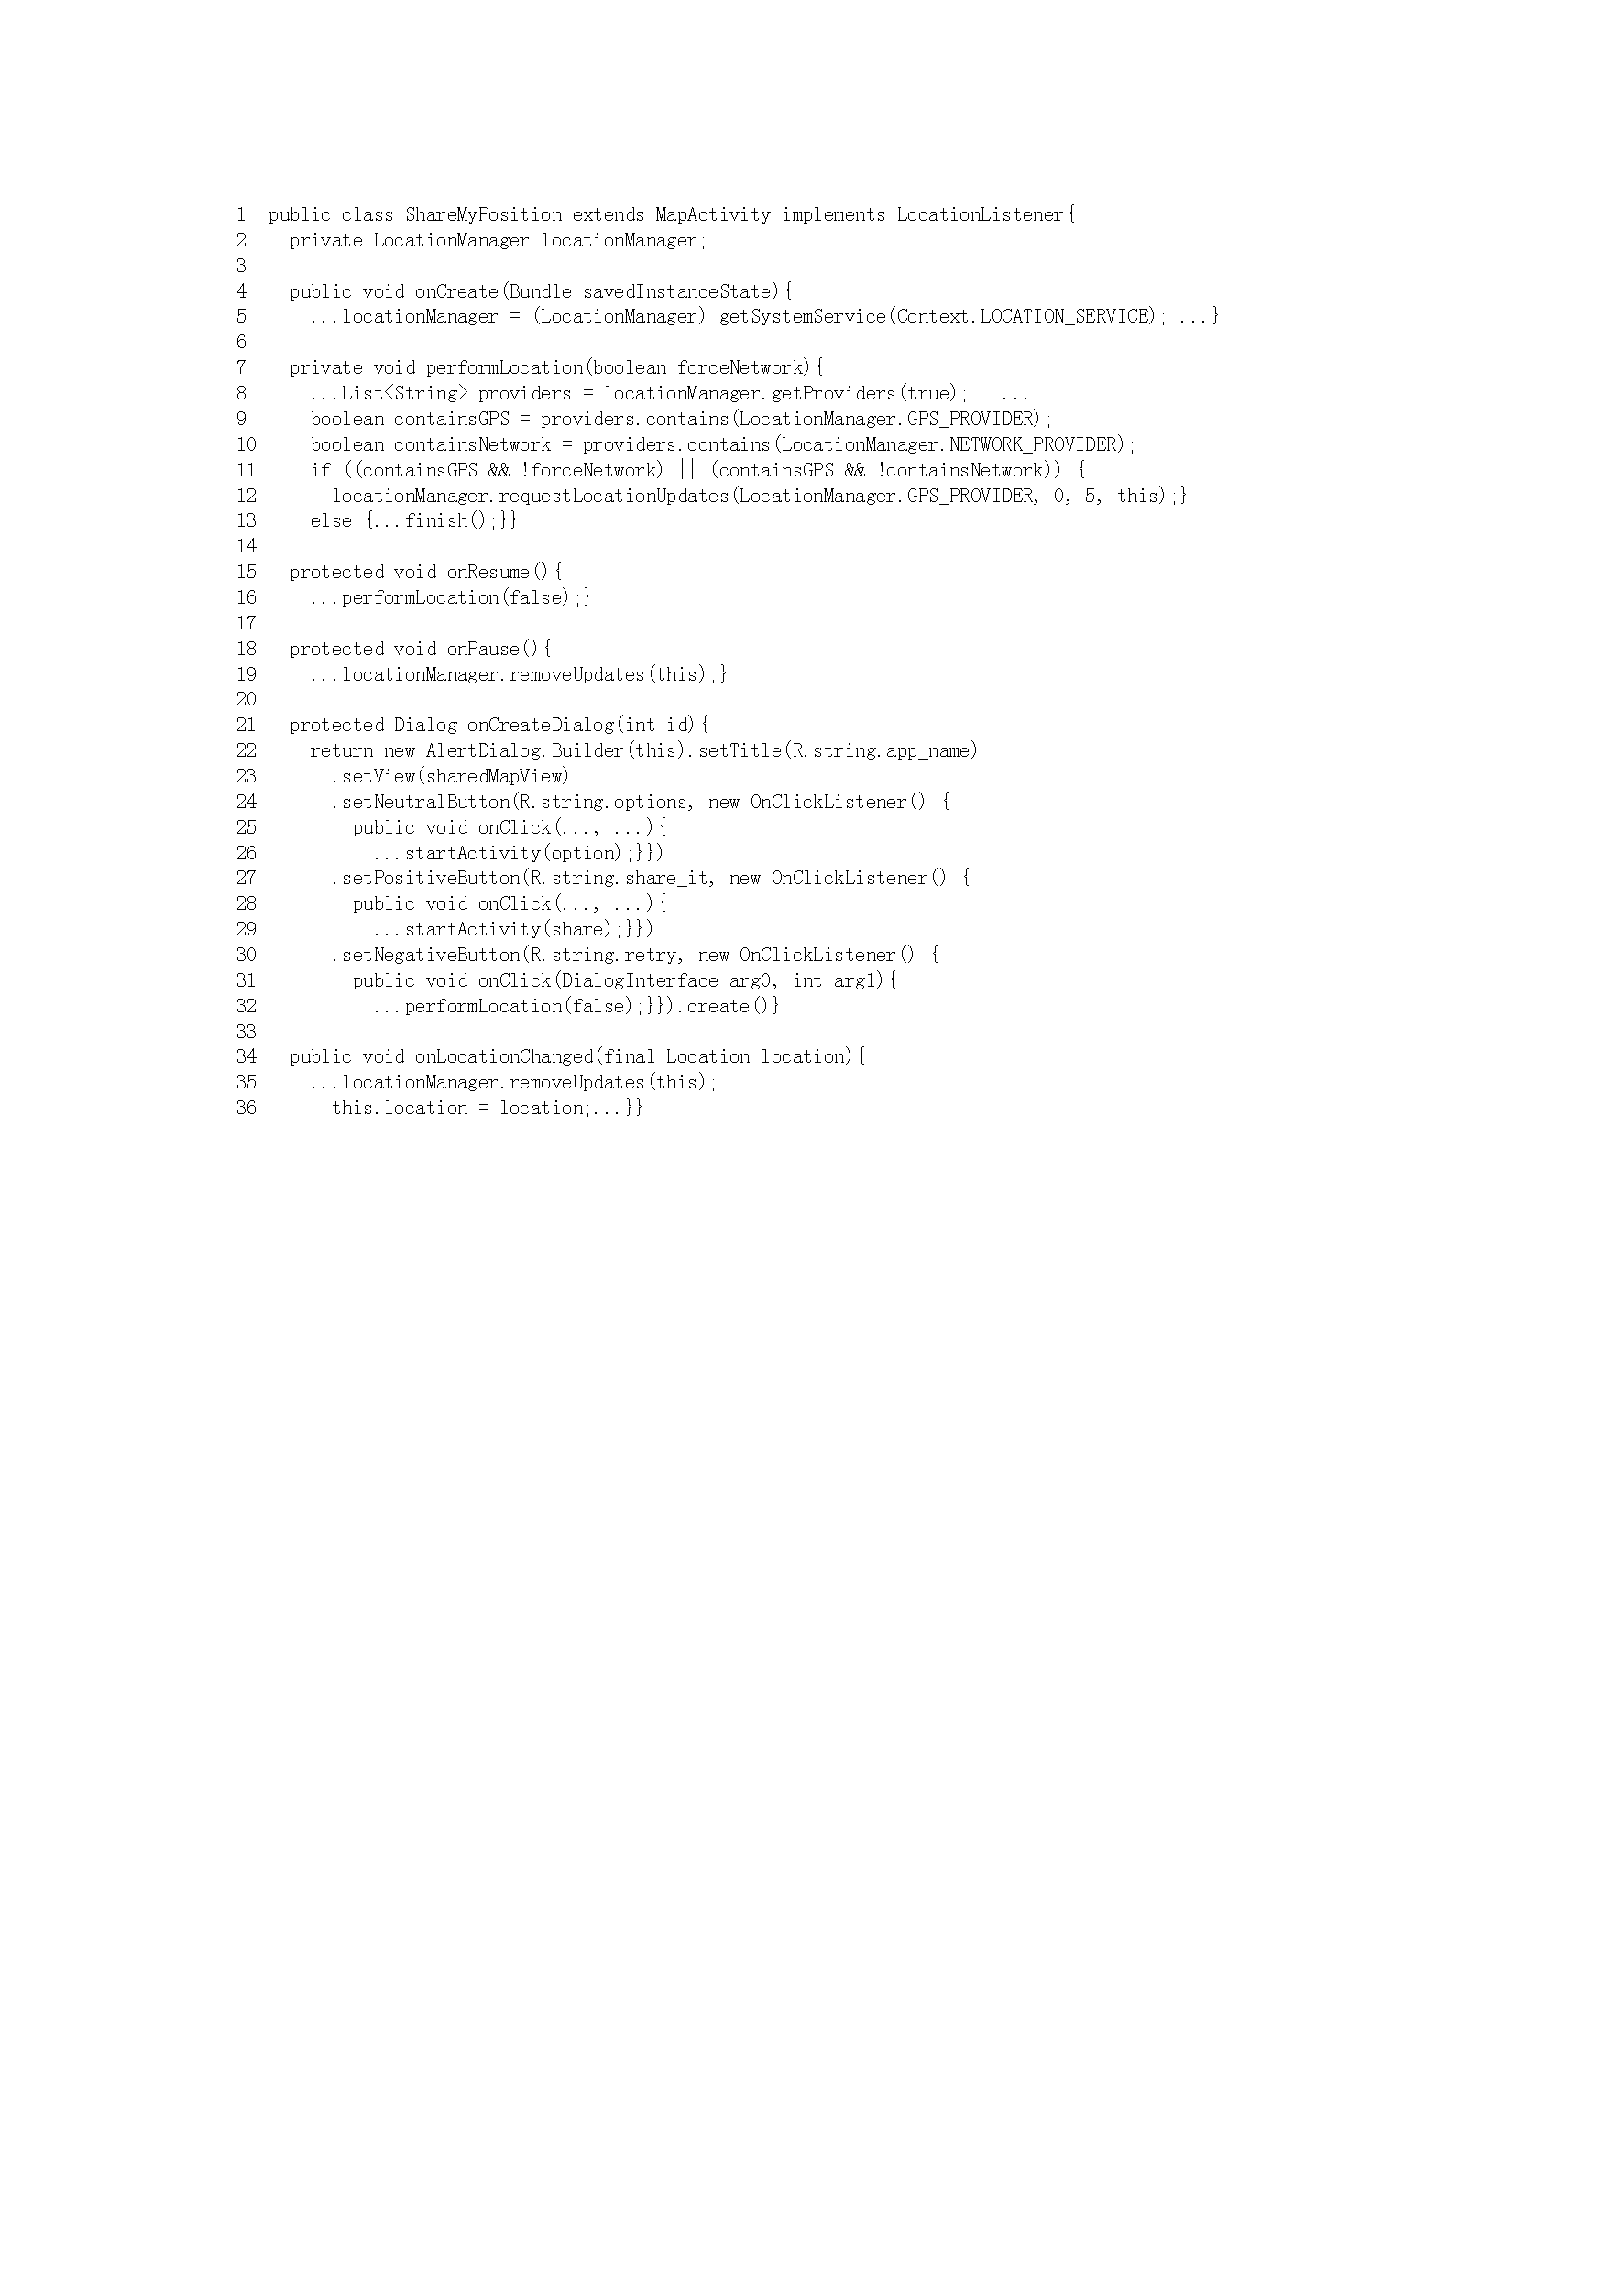
\includegraphics[width=1\linewidth]{pic/motivation1.pdf}  
  \caption{Motivation example derived from ShareMyPosition\cite{newShareMyPosition}.}  
  \label{fig:1}  
\end{figure}

The source code in Figure 1 is a fragment of app \emph{ShareMyPosition}, which is used to share a user's location to others. The main activity \texttt{ShareMyPosition} contains three lifecycle callbacks \big(\texttt{onCreate} (line $4$, $5$), \texttt{onResume} (line $15$, $16$) and \texttt{onPause} (line $18$, $19$)\big), as well as a system-driven callback \big(\texttt{onLocationChanged} (line $34-36$)\big). The main activity implements a listener interface \texttt{LocationListener} by overriding the method \texttt{onLocationChanged}. In the \texttt{onCreate} callback, ShareMyPosition defines and assigns a \texttt{LocationManager} type variable \texttt{locationManager}. Later in the \texttt{onResume} callback, the \texttt{locationManager} variable is used to register the callback listener \texttt{this} via a self-defined method \texttt{performLocation}. 
Rather than registering it directly, the \texttt{performLocation} first judges whether one of the conditions \texttt{containsGPS \&\& !forceNetwork} and \texttt{containsGPS \&\& !containsNetwork} is satisfied (line $11$). If so, the \texttt{this} object is registered as listener; otherwise, the lifecycle finishes. The system-driven callback \texttt{onLocationChanged} is activated along with the register action, but inactivated after the \texttt{this} listener is unregistered in the \texttt{onPause} or \texttt{onLocationChanged} callback. Besides of the system-driven callback, there exist three \textit{GUI} callbacks in function \texttt{onCreateDialog} (line $21-32$). These callbacks will be invoked when certain \textit{button-clicked} event fires. Particularly, the event on \textit{PositiveButton} (line $27-29$) and \textit{NeutralButton} (line $24-26$) will trigger a new activity.

 
\subsection{Problem Definition}\label{problem-define}
The example in Figure \ref{fig:1} causes challenges in traditional \textit{CCFG} (\textit{CCF} graph) construction. First, system-driven callback \texttt{onLocationChanged} is not directly invoked in the holder callback \texttt{onResume}. Whether it is invoked is determined by the calculation of several condition variables (\texttt{containsGPS}, \texttt{forceNetwork}, etc.). In the traditional \textit{CCFG}, these condition variables are ignored with the assumption that all the invoker can be connected with the invokee callbacks. However, this would result in significant confusion in traversing the callback flow model. Contrarily, a path-insensitive control flow generated by our method is more precise, since the variables are considered. 

Second, lifecycle callbacks in the example includes not only \texttt{onCreate}, but also
\texttt{onResume} and \texttt{onPause}. Traditional modelling methods handle the lifecycle callbacks in a coarse-grained way that only start (i.e., \texttt{onCreate}) and end (i.e., \texttt{onDestroy}) nodes are taken into consideration. Although it appears to be easy to handle the sequences of fine-grained callbacks like \texttt{onResume} and \texttt{onPause} among lifecycle callbacks, the modelling faces \textit{jumping confusion} once non-lifecycle callbacks are involved. For example, the \texttt{onClick} callback in line $28$ triggers the activity \texttt{share}, denoted as \texttt{PositiveButton.onClick} $\rightarrow$ \texttt{share.onCreate}. The \texttt{onPause} is known to be invoked when the current activity loses its focus, i.e., \texttt{onPause} should be invoked before \texttt{share.onCreate}. That is, the path \texttt{PositiveButton.onClick} $\rightarrow$ \texttt{ShareMyPosition.onPause} $\rightarrow$ \texttt{share.onCreate} is supposed to be created. However, if there exist a new path that leads to
\texttt{ShareMyPosition.onPause}, the path \texttt{ShareMyPosition.onPause} $\rightarrow$ \texttt{share.onCreate} should become invalid for the new path, e.g., the path \texttt{NeutralButton.onClick} $\rightarrow$ \texttt{ShareMyPosition.onPause} $\rightarrow$ \texttt{share.onCreate} should not be valid. Such situation that a node has multiple incoming and outgoing edges but not all combinations of incoming and outgoing edges form a valid path, is called jumping confusion, which makes jumping action between activities confusing and thus arises a challenge when considering callbacks like \texttt{onPause} in our model. Apart from jumping confusion, the fine-grained hybrid model would result in other unexpected conflicts between lifecycle and non-lifecycle callbacks. For instance, assuming that an \texttt{onClick} callback is registered in the \texttt{onCreate} callback, there should be an edge connecting the two callbacks. However, this edge would become invalid when encountering \texttt{onResume}, since the \texttt{onResume} should always be first invoked after the \texttt{onCreate}.

Another challenge in the \textit{CCFG} construction is the representation of inter-components, which is not explicitly presented in the motivation example. As mentioned in Section \ref{background}, the objective component in the inter-components jumping can be either service or activity. The jumping for activity can be treated as normal control flow since the invoker and invokee occur one after another. For the service, however, the jumping only acts as a launcher for triggering the objective component. There is not a strict chronological order between invoker and invokee in service case, because service runs in a parallel with other components. Due to the above differences, a fine-grained modelling has to distinguish the two types of jumping.

%Apart from activity, other three domain components: service, broadcastReceiver and content provider also play important roles in constructing general callback model. Similar with the jumping between activities, the transition between different components types is also under a certain container callback within the previous component. However, the program of different components can be executed in a parallel way. For example, a service is able to running in background at the time a foreground activity in the same app is active. Thus the traditional control flow graph is hard to represent the program logic between components of different types. Especially, component like service has its own lifecycle as activity does. Completely considering every status appears quite challenging. To this end, we propose a novel representation to describe the generic model, especially for the model across components, within an app. We introduce this representation in section \ref{transition-model}.

%\textbf{Path-sensitive}. Considering \textit{path-sensitive} within target program benefits a lot for the precision of control flow analysis\cite{}. Traditional callback models \cite{} are seldom considering path-sensitive, leading to the generated model just works as a architecture reflection for aided analysis. That is to say, a path-insensitive model could not directly be used for applied testing, verification or security analysis, causing these techniques need more flow details guiding the execution. In our example, whether the \texttt{onLocationChanged} is active or not is dependent on the predicates at conditional branch instructions. If the modelling discards considering the branch predicates, it is impossible to distinct whether the callback fires in an absolute way under its container callback(\texttt{onResume} in this case) or not. Such details could directly impact processing of high-level techniques upon the generated model, such as generation of test case (for testing) and logic properties (for model verification and security analysis).

%We address the path-sensitive challenges using data dependency analyses introduced in section \ref{path-sensitive}. 
  
%\textbf{Fine-grained lifecycle}
%Handling fine-grained lifecycles like \texttt{onResume} and   \texttt{onPause} is of importance for constructing a complete callback model. For the processing of system listener register, the register and unregistered sentences are often located in \texttt{onResume} and \texttt{onPause} callbacks. Therefore, analysis towards these lifecycle callbacks is indispensable.

%Usually, these sorts of callbacks are designed to be invoked in some specific time according to the activity's running status, e.g., losing focus or recovering focus. Each time when current activity jump to a new one, the fine-grain lifecycle like \texttt{onPause} and \texttt{onStop} will be invoked in sequences. Since the destinations of activity jumping may be different (e.g., the \texttt{share} and \texttt{option}), it has to generate two different paths for the two jumping. However, both of the two paths contain the same fine-grained lifecycle callbacks. One simple tackling manner is to generate a copy fine-grain lifecycle for each path, but it can yield redundancy nodes and edges, which will impact the traverse cost and model precision. So how to generate a reasonable model which can properly handle the fine-grain lifecycle callbacks becomes a challenge. We propose our solution in section \ref{fine-grain lifecycle}.

%\section{Generic Path-sensitive Callback Model}\label{transition-model}
In this section, we introduce the GPC model and define related conceptions. 

\textbf{Definition 1.} A \textit{Generic Path-sensitive Callback Model} (GPC) is a tuple
\begin{equation}
GPC = (N, E, C)
\end{equation}
%consisting of the followings.
\begin{itemize}
\item \textit{N} is the set of nodes, representing the set of callbacks. \textit{N} contains two parts and is denoted as $ N = N_{l}\cup N_{n}$.  $ N_{l}$ refers to the set of lifecycle callbacks and can be divided into two parts, $N_{l}= N_{lfc}\cup N_{aux}$, in which $N_{lfc}$ and $N_{aux}$ refer to the set of system and auxiliary lifecycle. Auxiliary node set $N_{aux}$ is added into lifecycle modelling for auxiliary analysis. $N_{aux}$ contains three defined callbacks \textit{ActiveStart}, \textit{ActiveEnd} and \textit{Terminal}, denoted as $N_{aux} = \{N_{as}, N_{ae}, N_{tm} \} $. Correspondingly, $N_{n}$ refers to the set of non-lifecycle callbacks. $N_{n} = N_{sys}\cup N_{gui}$, in which $N_{sys}$ and $N_{gui}$ refer to the set of system and \textit{GUI} callbacks. We denote the nodes of component \textit{x} as $N^{x}$, the set of start node as $N_{st}$ and the set of restart node as $N_{re}$. 
\item \textit{E} is the set of edges that represents the invocation sequence between two nodes. \textit{E} can be generated via three ways: lifecycle event, register action and inter-component jumping. We denote them as $E = E_{l}\cup E_{r}\cup E_{j}$, in which $ E_{l} = N_{l} \times N_{l}$ , $ E_{r}  = (N_{l} \times N_{n}) \cup (N_{n} \times N_{l}) \cup (N_{n} \times N_{n})$ and $ E_{j} = E_{j-a}\cup E_{j-s} = (N_{tm}^{A} \times N_{st}^{B}) \cup (N_{tm}^{B}\times N_{re}^{A})$, where $E_{j-a}$ refers to the inter-component edges between activities; $E_{j-s}$ refers to the ones involving service component, $~^A$ and $~^B$ refers to any two components.
\item \textit{C} is the set of conditions for nodes, $C = \{( r, f, e )| r\in Ivr, f\in \Lambda, e\in Ive\}$ where \textit{Ivr} refers to the set of invoker callbacks; \textit{Ive} is the set of invokee callbacks; $\Lambda$ is the set of conditions where each element is a boolean expression with variables. Formally, $\forall f\in \Lambda, f : Val \rightarrow \{True, False\}$, where \textit{Val} is the assigned values of variables.
\end{itemize}

\textbf{Definition 2.} \textit{Register Abstraction} (\textit{RA}) is the set of actions for register (\textit{FRA}) and unregister (\textit{BRA}) of the non-lifecycle callbacks, which is denoted as a set of tuple
\begin{equation}
RA = \{( r, g, e) |r\in Ivr, g\in \Gamma, e\in Ive\}
\end{equation}
%consisting of the following elements:
\begin{itemize}
\item \textit{Ivr} and \textit{Ive} refer to the set of invoker and invokee callbacks respectively.
\item $\Gamma$ refers to set of register (for \textit{FRA}) and unregister (for \textit{BRA}) actions. Each element in $\Gamma$ contains two parts: object and API, namely $\forall g \in \Gamma, g = (obj, API)$, meaning that the object conducts (un)register action and the API is employed by the object.
\end{itemize}

Take the motivation example for illustration. The \textit{FRA} modelling the register action in line $12$, is \texttt{(onResume,\linebreak
(locationManager,requestLocationUpdates), onLoc-\linebreak ationChanged)}; the \textit{BRA} for the unregister action in line $19$, is \texttt{(onPause,(locationManager,removeUpdates), onLocationChanged)}.



\textbf{Definition 3.} \textit{Jumping Abstraction} (\textit{JA}) is the action that launches (\textit{FJA}) and terminates (\textit{BJA}) new component \textit{B} from current running component \textit{A}, denoted as a set of tuple 
\begin{equation}
JA = \{( r, u, e )| r\in Ivr^{A}, u\in \Upsilon, e\in Ive^{B}\}
\end{equation}
%consisting of the following elements:
\begin{itemize}
\item For \textit{FJA}, $Ivr^{A}$ and $Ive^{B}$ refer to the launcher callback in \textit{A} and the launched callback in \textit{B} respectively.
Correspondingly, for \textit{BJA}, \item $Ivr^{A}$ refers to the callback in \textit{A} for terminating \textit{B}; and $Ivr^{B}$ refers to the callback in \textit{B} terminated by \textit{A}.
\item $ \Upsilon$ refers to the set of jumping actions in the invoker component (i.e., \textit{A}). Similar as \textit{RA}, each element in $\Upsilon$ also contains the object and API, namely $\forall u\in \Upsilon, u = (obj, API)$, which refers to the jumping object and employed API.
\end{itemize}

In the motivation example, as for the jumping action in line $29$, the jumping abstraction can be denoted as \texttt{(ShareMyPosition\$2}$::$\texttt{onClick,(ShareMyPosition.\linebreak this,startActivity),share}$::$\texttt{onCreate)}. Note that \texttt{ShareMyPosition\$2} is the inner anonymous class of \texttt{ShareMyPosition}, which contains the invoker \texttt{onClick}.


The \textit{RA}, \textit{JA} and the lifecycle flow set (\textit{LF}) are three key types of connections between callback nodes. The \textit{GPC} edges are generated by identifying these flow sets. The relation between the defined connections and edges are:
 $RA$ mapping to  $E_{r}$,
 $JA$ mapping to  $E_{j}$, and
 $LF$ mapping to  $E_{l}$.

\textbf{Definition 4.} \textit{Event} is the situation that triggers the invocation of callback, which is denoted as a set of tuple
\begin{equation}
Event = \{( t, a, o )| t\in Tgr, a\in Act, o\in Obj)\}
\end{equation}
%consisting of the following elements:
\begin{itemize}
\item \textit{Tgr} refers to the set of objects that conduct a trigger action. An element in \textit{Tgr} has two selectable items: \textit{user} and \textit{system}.
\item \textit{Act} refers to the set of trigger actions. Typical elements in \textit{Act} include \textit{Click}, \textit{Touch}, \textit{LocationChanged}, etc.
\item \textit{Obj} refers to the set of triggered object. Typical elemenents in \textit{Obj} include instances of \textit{Button}, \textit{View}, \textit{LocationManager}, etc.
\end{itemize}

\textbf{Definition 5.} \textit{HiddenNodes} represents the unimplemented lifecycle callbacks in the target app. The \textit{hiddenNodes} set can be computed by the formula
 $HiddenNodes = ELG.nodes - N_{l} $, where \textit{ELG.nodes} is the entire lifecycle nodes.

\textbf{Definition 6.} \textit{Active Area} is a lifecycle interval where the non-lifecycle callbacks are normally invoked.

The active area is quite different in activity and service. For activity, the active area is located between \texttt{onResume} and \texttt{onPause}; for service, it is located between \texttt{onStartCommand} and \texttt{onDestroy}, or between \texttt{onBind} and \texttt{onUnbind} (for service with \texttt{onbind} callback). The auxiliary nodes \textit{onActiveStart} and \textit{onActiveEnd} are initialized to identify the active area. For instance, a partial picture of activity's lifecycle model is  $\texttt{onResume}\rightarrow \texttt{onActiveStart}\rightarrow \texttt{onActiveEnd}\rightarrow \texttt{onPause}$.
We do not consider the extreme situation where non-lifecycle callbacks are invoked outside the \textit{Active Area}.

\section{Construction Algorithm}\label{algorithms}

%Android uses observer pattern to handle both user-driven and system-driven callbacks, namely non-lifecycle callbacks according to section \ref{background}. A non-lifecycle callback (termed as \begin{math} \mathcal{C} \end{math}) becomes valid only when its container listener is properly registered. Whereas the register process(termed as \begin{math} \mathcal{R} \end{math}) is located in another container callback (termed as \begin{math} \mathcal{P} \end{math}). 
%Define 0 callback status  (inactive, active, invoked)
%Define 1 register-triple
%The triple (\begin{math} \mathcal{P},\mathcal{R},\mathcal{C} \end{math})) named register-triple performs the key flow relations between callbacks, where the register process acts as a bridge connecting with two callbacks. Figure 2 illustrates the register-triple within the motivating example. ... Then we can define a generalized connection triple.
%Define 2 connection triple
%connection triple = register-triple + ICC connection

%\begin{figure}[!t]  
%  \centering  
%  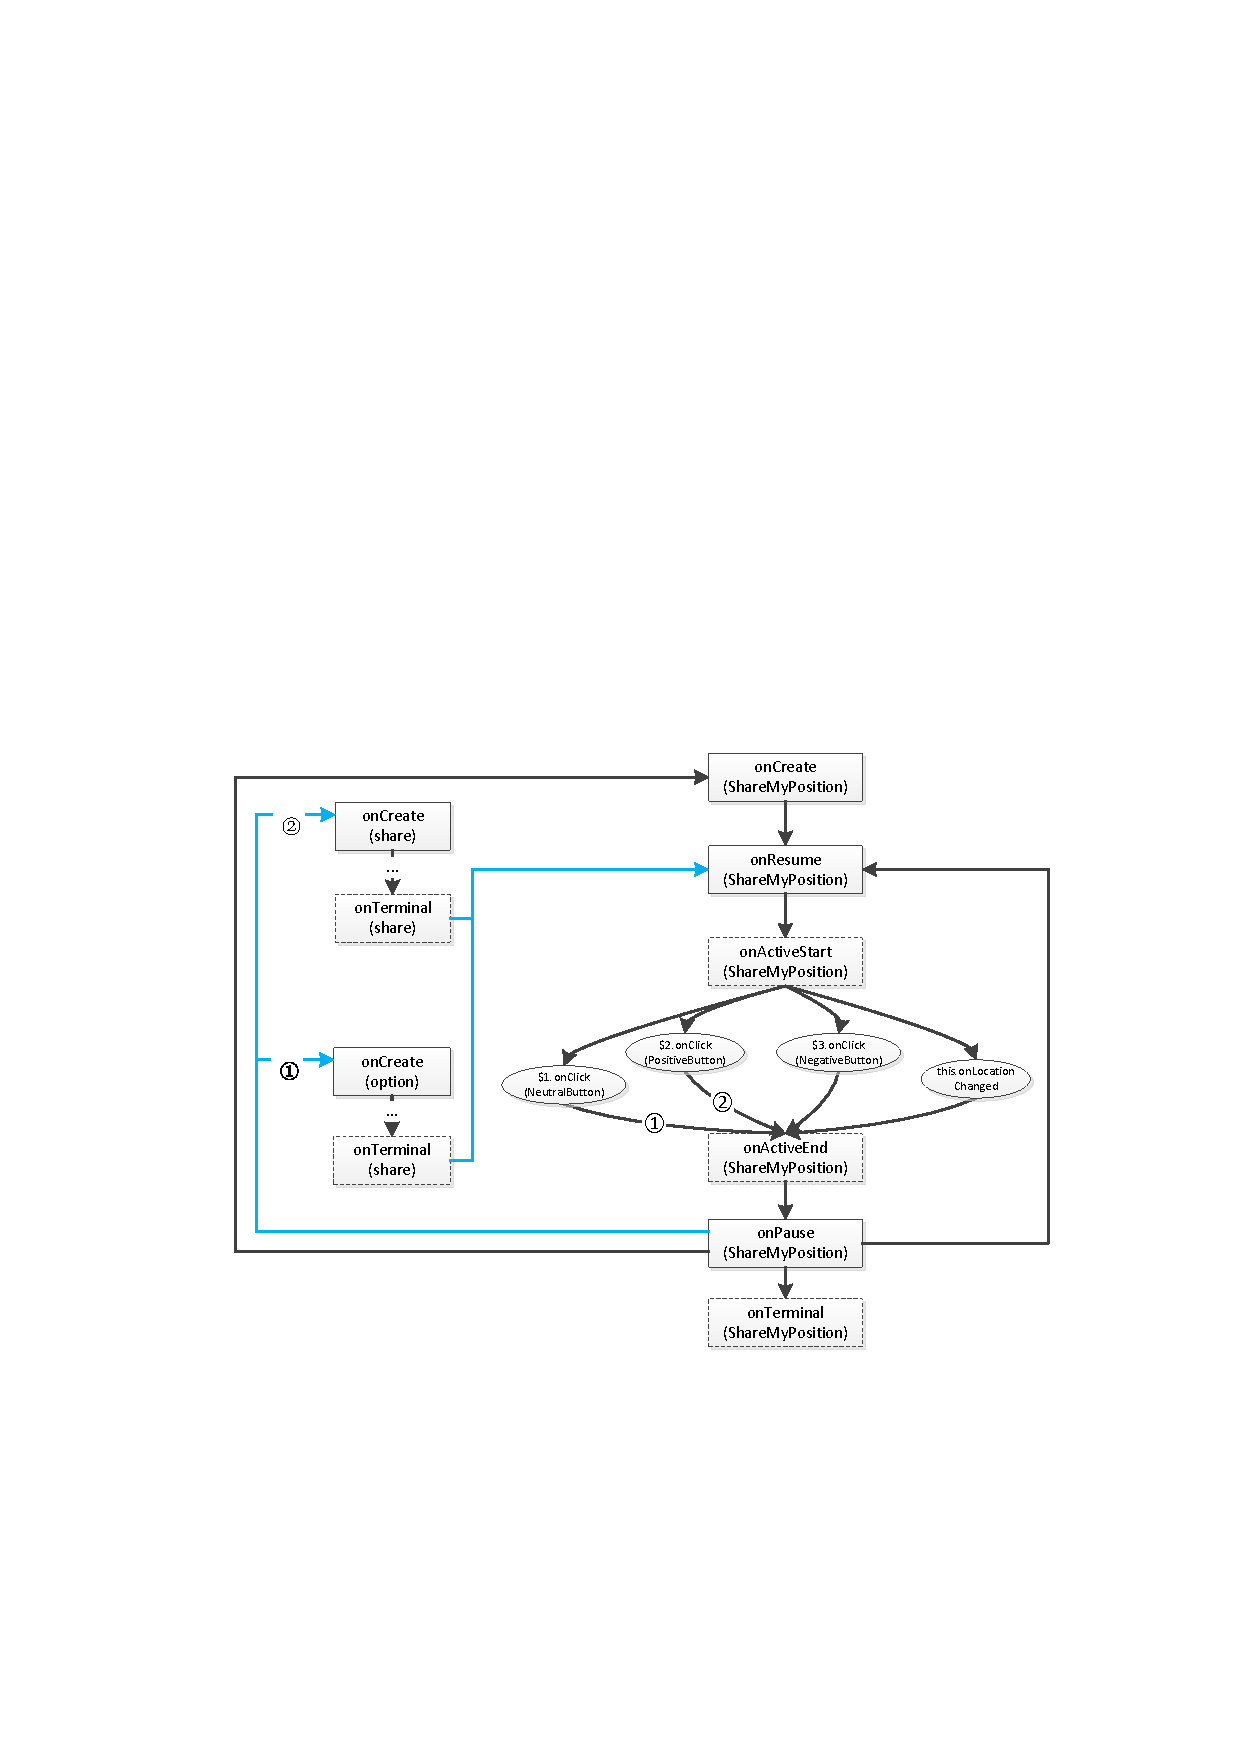
\includegraphics[width=1\linewidth]{pic/motivationGPM.pdf}  
%  \caption{GPC model illustration for motivation example.}  
%  \label{fig:motivationGPC}  
%\end{figure}

\begin{table*}[!t]
\centering
\begin{threeparttable}[b]
\caption{Path-sensitive conditions for motivation example. } 
\newcommand{\tabincell}[2]{\begin{tabular}{@{}#1@{}}#2\end{tabular}}
\small
\begin{tabular}{|c|c|c|c|c|}
\hline 
Node & Connection & ConType & Condition & Event\\ 
\hline 
\hline 
this.onCreate & \$1$::$onClick & FRA & N/A & env:(user,click,NeutralButton) \\ 
\hline 
this.onCreate & \$2$::$onClick & FRA & N/A & env:(user,click,PositiveButton) \\ 
\hline 
this.onCreate & \$3$::$onClick & FRA & N/A & env:(user,click,NegativeButton) \\ 
\hline 
this.onResume & this.onLocationChanged & FRA & \tabincell{c}{con:((v1 \&\& !v2)$\parallel$ \\
(v1 \&\& !v3))} &  env:(sys,locationChanged,locationManager)\\

\hline 
this.onPause & this.onLocationChanged & BRA & N/A & N/A \\ 
\hline 
this.onLocationChanged & this.onLocationChanged & BRA  & N/A & N/A \\ 
\hline 
\$1$::$onClick & option$::$onCreate & FJA  & N/A & N/A \\ 
\hline 
\$2$::$onClick & share$::$onCreate & FJA  & N/A & N/A \\ 
\hline 
\end{tabular}
\begin{tablenotes}
    \item [1] The signs \textit{v1}, \textit{v2} and \textit{v3} in column \textit{Condition} respectively refer to the variables \textit{containsGPS}, \textit{forceNetwork} and \textit{containsNetwork}
   \end{tablenotes}
\label{tbl: sensCond}  
\end{threeparttable}
\end{table*}
In this section, we introduce the \textit{GPC} construction algorithms, %Figure \ref{fig:motivationGPC} describes the \textit{GPC} model for the motivation example. 
including the following four stages.
%: 1) constructing path-insensitive inner component model, 2) constructing inter-component model, 3) constructing path-sensitive model and 4) handling fine-grained flow. %Correspondingly in Figure \ref{fig:motivationGPC} and Table \ref{tbl: sensCond}, the construction stages can be clearly mapped as: 1) constructing all the nodes and black edges; 2) constructing the blue edges; 3) obtaining the \textit{Conditions} column in Table \ref{tbl: sensCond}; 4) building the order numbers on Figure \ref{fig:motivationGPC}'s edges. Our approach is based on static analysis techniques. The input of our analysis algorithm is the app byte codes via reverse engineering. The output is the generated \textit{GPC} model, including the set of nodes, edges and conditions. Related conceptions have already been defined in Section \ref{transition-model}. 
%A conditionEdge can be a ordinary edge or the edge with trigger conditions that contains two parts: register conditions and trigger events.

\subsection{Path-insensitive Inner Component Model (\textit{PII})}
In this stage, we present a process\textit{ConsPII}. Taking the source code of a target component as its input, the process 
outputs a path-insensitive model for the component, including valid nodes (set \textit{N}) and edges between the nodes ($E_{l} \cup E_{r}$ -- lifecycle edges $E_l$ and register edges $E_r$).
%thow to construct the set of valid nodes \textit{N} and the set of edges $E_{l} \cup E_{r}$ (lifecycle and register edges) in each component. We call this process \textit{ConsPII}. As an improved static analysis, the algorithm takes the source code of the target component as its input. The output of \textit{ConsPII} is a path-insensitive model for target component, including valid nodes and edges. Since the set of nodes \textit{N} can be easily identified by matching pre-defined regular expression, \textit{ConsPII} focuses on constructing valid edges, namely the lifecycle edges $E_{l}$ and the register edges $E_{r}$.  

The nodes in \textit{N} are identified by matching pre-defined regular expression.
To compute $E_{l}$, \textit{ConsPII} first initializes an entire lifecycle graph (\textit{ELG}) in accordance with the type of the given component. Then, three \textit{auxiliary nodes} (\textit{onActiveStart}, \textit{onActiveEnd} and \textit{onTerminal}) are created and added into the ELG. They are used to explicitly mark the component status. \textit{ConsPII} then identifies the implemented lifecycle callback in the given component. For the nodes in the \textit{ELG} that are not implemented in the component, \textit{ConsPII} employs a displacement algorithm in the ELG, which involves three steps: 1) checking the pre-nodes and post-nodes of the unimplemented nodes, 2) generating edges connecting each pre-node with each post-node, 3) removing the unimplemented and its related edges. After the displacement, the $E_{l}$ is obtained from the remaining edges of ELG. 

%The $E_{r}$ are generated via identification of (un)register abstractions (\textit{RA}, defined in Section \ref{transition-model}).
To identify the edges in $E_r$, we first identify a set of register actions $\mathit{FRA}$, then the \textit{ConsPII} process adopts an improved \textit{DFS} (Deep First Search) algorithm over the entire program. The traversal process starts with \texttt{onCreate} callback in the launcher activity. For each identified register action $\mathit{fra}\in \mathit{FRA}$, the invokee callback \textit{ive} is taken as a new node and is inserted into \textit{active area} -- a lifecycle interval where the non-lifecycle callbacks are normally invoked. The \textit{active area} is defined for addressing the conflicts between lifecycle and non-lifecycle callbacks, and located between two auxiliary nodes: \textit{onActiveStart} and \textit{onActiveEnd}. There are two types of connections: \textit{lifecycle} $\rightarrow $ \textit{non-lifecycle} and \textit{non-lifecycle} $\rightarrow $ \textit{non-lifecycle}. The former generates edges \textit{onActiveStart} $\rightarrow $ \textit{ive} $\rightarrow $ \textit{onActiveEnd}; while the latter generates edges \textit{ivr} $\rightarrow $ \textit{ive} $\rightarrow $ \textit{onActiveEnd}, where \textit{ivr} is the invoker in the \textit{fra} tuple. %The black arrows and all the nodes in Figure \ref{fig:motivationGPC} are generated by \textit{ConsPII}. Note that in the figure, the \textit{onCreateDialog} is substituted by the \textit{onCreate}, since \texttt{onCreateDialog} is always invoked along with \textit{onCreate}, and thus can be treated as a part of it.

%\begin{algorithm}[!t]
%\caption{Connection between Components}
%\footnotesize
%\begin{algorithmic}[1]
%\Procedure {ConsPII} {$comp$}
%\State $ELG \leftarrow constructLifecycleGraph(comp)$
%\State $ auxNodes \leftarrow geneAuxNodes(comp)$
%\State $    nodes \leftarrow ELG.nodes$
%\State $    edges \leftarrow ELG.edges$
%\State $     lifeNodes, nonLifeNodes \leftarrow getAllValidCallbacks()$
%\ForAll {$hiddenNode \in (ELG.nodes \setminus lifeNodes)$}  
%\State $        edges \leftarrow edges \cup geneEdges(hiddenNode.preNodes,$\\
% $\ \ \ \ \ \ \ \        hiddenNode.postNodes)$
%\State $        nodes \leftarrow nodes \setminus hiddenNode$
%\State $        edges \leftarrow edges \setminus hiddenNode.edges$
%\EndFor

%\State $ FRA \leftarrow getRA(comp)$
%\ForAll {$ fra \in FRA $}
%\If {$fra.ivr\in lifeNodes\ \&\&\ fra.ive\in nonLifeNodes $}
%\State $            nodes \leftarrow nodes \cup fra.ive$
%\State $            edges \leftarrow edges \cup geneEdge(auxNodes.activeStart, fra.ive)$
%\State $            edges \leftarrow edges \cup geneEdge(fra.ive, auxNodes.activeEnd )$
%\ElsIf{$ fra.ivr\in nonLifeNodes\ \&\&\ $\\
% $\ \ \ \ \ \ \ \ \ \ \ \ \ \ \ \ \ \ fra.ive\in nonLifeNodes $}
%\State $  nodes \leftarrow nodes \cup fra.ive$
%\State $  edges \leftarrow edges \cup geneEdge(fra.ivr, fra.ive)$
%\State $  edges \leftarrow edges \cup geneEdge(fra.ive, auxNodes.activeEnd )$
%\Else {$ pass$}
%\EndIf
%\EndFor
%\EndProcedure
%\end{algorithmic}
%\label{fig:alg1}
%\end{algorithm}


%We use an improved DFS algorithm to traverse all the program source code (some irrelevant contents are excluded) and recognize the triple structure. The traversal process starts with the \texttt{onCreate} callback of launcher activity. First, system constructs a raw lifecycle model according to the lifecycle structure. This process is quite trivial. Then all the lifecycle callbacks in the raw model will be regarded as sub-roots, and each sub-root generates a flow-tree by linking the recognized the \textit{connection triple}. In this stage, we get a rough path-insensitive, control flow model. In this model, each callback acts as a node, and each connection triple acts as an edge.

%1) Checking register triple. Register triple determines when and where a callback becomes valid , as well as the connection between two related callbacks, especially the system-driven and user-driven callbacks. Checking the register triple is to find the execution sequences via traversing the program source code.

%2) Path-insensitive Inner Component Model. Inner component model acts as topology callback sequence without considering the connections of different components and jumping conditions. Constructing such model needs to well tackle the invocation order between lifecycle callbacks and other callbacks. Callback model generated in this step is able to represent fine-grained and complete callback sequences for each component.

%Algorithm 1 presents the analysis to detect registered actions. It essentially iterates over all program entry points (EntryPoints) and all actions (Action-Set) supported by the mobile framework (lines 6 􀀀 16). For each entry point P and action X it extracts the call graph of the app (line 5) and locates a set of statements PNodeSet (line 8) containing instances of a valid event-listener registering statement L for action X. Finally, for each statement PNode in PNodeSet it performs a backward slice on PNode to locate an initialization statement of the widget on which the instance of L was called (lines 10􀀀12). This is used to get an identier ID of the component (line 13) which is registered in the action map E with the action X.

\subsection{Connections between Components (\textit{CBC})}
Connections between components can be divided into two types: \textit{sequential jumping} and \textit{parallel jumping}. The former represents the invokee that occurs after the end of invoker. \textit{Sequential jumping} normally exists in the connections between activities, since the activities occupy the foreground (in running status) in sequence of invocation. The latter occurs when service involves, because a service runs in the background in parallel with the foreground activity or other services.

The process for constructing the connections is called \textit{ConsCBC} (Constructing the \textit{CBC}). \textit{ConsCBC} takes the sequential jumping as normal edges in \textit{PII}. As for parallel jumping, \textit{ConsCBC} generates specialized \textit{parallel edges} to represent the parallel relationship since it is beyond the representation of \textit{PII} and traditional \textit{CFG}. Typically, \textit{ConsCBC} considers the end connections (e.g., stopService, unbindService) as well as the start connections (e.g., startService, bindService). Specifically, if the trigger component is an activity, we define \textit{parallel slice} by the slice of a trigger activity model that can run in parallel with the service. For example, service \textit{S} is launched and stopped in activity \textit{A} via the API \texttt{startService} and \texttt{stopService}. Thus, only the nodes that can run between \texttt{startService} and \texttt{stopService} are possible to run in parallel with service \textit{S}. The paths consisting of such nodes and related edges in \textit{A} are treated as \textit{parallel slice}. The parallel slice provides a fine-grained picture for better understanding the parallel relation between the invoker and invokee. Algorithm \ref{fig:alg2} handles the parallel slice in line $16-25$. The algorithm traverses all the feasible paths that contain startNode (e.g., startService) and checks the paths that contain endNode (e.g., stopService) as well. Then, the algorithm marks the checked nodes as parallel slice nodes. Note that in parallel jumping, if the service is terminated by itself, the parallel slice will act as the entire \textit{PII} of trigger activity.

%\begin{algorithm}[!t]
%\caption{Path-insensitive Inner Component Model Construction}
%\footnotesize
%\begin{algorithmic}[1]
%\Procedure {ConsCBC} {$PII$, $connStSet$, $connEndSet$}
%\State $//Generate\ startConnection\ between\ component$
%\ForAll {$connSt \in connStSet$}  
%\If {$connSt\in activity\rightarrow activity$}
%\State $        geneEdge(connSt.holderNode, newCompEntry)$
%\ElsIf {$   connSt\in (comp \rightarrow service || service \rightarrow comp)  $}
%\State $        geneParallelEdge(connSt.holderNode, newCompEntry)$
%\Else $pass$
%\EndIf
%\EndFor
%\State $ //Generate\ endConnection\ between\ component $
%\ForAll {$ connEnd \in connEndSet $} 
%\State $  geneParallelEdge(service.end, connEnd.holderNode )$
%\EndFor    
%\State $ connPairSet\leftarrow Set(connSt.holderNode,connEnd.holderNode)$
%\State $       //Mark\ the\ parallel\ slice$
%\ForAll {$ connPair\in connPairSet$}
%\State $  pathsSt \leftarrow getPaths(connPair.startNode)$
%\ForAll {$ path in pathsSt $}
%\If { $ path.contains(connPair.endNode) $ }
%\State $   sliceNodes \leftarrow sliceNodes \cup path.nodes$
%\EndIf
%\EndFor
%\EndFor
%%\State $   // sliceNodes \leftarrow getSliceNodes(connPair)   //complexity\ is\ O(e)$
%\State $       markSliceNodes(sliceNodes )$
%\EndProcedure
%\end{algorithmic}
%\label{fig:alg2}
%\end{algorithm}


%Components of different types can be executed in parallel, which is beyond the representation of existing modelling approaches. For example, if a service \textit{s} is launched by an activity \textit{a}, the \textit{s} will run it program logic in background, and this time the foreground \textit{a} continues its running. 

%The GPC model can represent this relationship through \textit{parallel slice} of the trigger component. The \textit{parallel slice} is from a trigger node to a close node, which respectively trigger other component active and destroy. The triggered component only can be executed parallel with the logic with \textit{parallel slice} of the trigger component. Some components are triggered or closed by themselves. For example, a statically registered broadcastreceiver is triggered when the app starts; a service destroys its process by itself. The \textit{parallel slice} of activities (if any) for these components are the entire activities program. GPC model uses different flags to sign the different \textit{parallel slices}.

%3) Connections of Components. The generated models by steps 2 aiming to single component can not reflect invocation relations for entire app program. The connections of components focuses on both new component trigger and stop. Especially, in connecting with the parallel (可并行的) component like service, the specific \textit{parallel slice } is computed through the feasible path nodes between trigger and stop point.

\subsection{Path-sensitive Inter-component Model (\textit{PSI})} 
The \textit{PII} and \textit{CBC} lack identification for trigger conditions, which heavily limits the available area. To address this issue, a path-sensitive modelling approach called \textit{ConsPSI} (constructing the \textit{PSI}) has been proposed, as shown in Algorithm \ref{fig:alg3}. Essentially, \textit{ConsPSI} aims at handling the trigger conditions for registering edges $E_{r}$ and inter-component connections $E_{j}$. Lifecycle edges $E_{l}$ need not to be handled since they are triggered without extra conditions. For each edge in $E_{r}$ and $E_{j}$, the path-sensitive model represents the condition set under which the invokee callback is fired. To achieve this goal, \textit{ConsPSI} engages a backward data dependency analysis for critical program slice, which involves two core analyses: \textit{checkCV} (for checking the condition variables) and \textit{backTraverse} (for tracking the condition values). Since \textit{ConsPSI} uses the same methods to handle $E_{j}$ as to handle $E_{r}$, we only describe how to handle $E_{r}$ for simplification.

The goal of \textit{checkCV} is to check the trigger conditions for callback invocation and to record variable set within such conditions. The checked objects intuitively originate from the register action (\textit{rAct}) contained in \textit{FRA}, because the invocation of a non-lifecycle callback heavily relies on execution of the \textit{rAct}. For each $fra\in FRA$, \textit{checkCV} identifies the \textit{rAct} branch using backward matching, and then records the branch conditions. In essence, \textit{checkCV} abstracts all the variables within the branch conditions and preserves them in a maintained list \textit{CVList}.

The \textit{backTraversal} for variable dependency analysis is based on the \textit{CVList} obtained by \textit{checkCV}. The goal for \textit{backTraversal} is to clarify the values of condition variables. To this end, \textit{backTraversal} backward tracks the variable assignment to update the \textit{CVList}. The atomic unit of \textit{CVList} is a variable tuple $\textit{vt} = (var, val)$, where \textit{var} and \textit{val} refer to the name and value of the variable. The \textit{val} can be either a \textit{vt} set or a terminal value. The tuple \textit{vt} keeps evolving during variable tracking. Eventually, all the \textit{val}s in \textit{vt} are updated to terminal values. The evolving process of motivation example is shown in Figure \ref{fig:motConds}. Leaves \textit{vt}s (blue nodes) in Figure \ref{fig:motConds} only contain terminal values. Typically, \textit{backTraversal} records three types of leaf \textit{val} at the end of tracking: constant value, \textit{PARA} and \textit{GLOBAL}. \textit{PARA} and \textit{GLOBAL} represent the parameter type and global type of \textit{var}, respectively. When the tracking ends in a method, the \textit{val} is still possible to be an undetermined variable. \textit{backTraversal} identifies the types of these variables and marks them as \textit{PARA} or \textit{GLOBAL}. The implementation process of \textit{backTraversal} is shown in Algorithm \ref{fig:alg3} line $4-11$. Eventually, the final results stored in \textit{pathSens} are treated as an attribute of the invoker node in $fra$.

%For each item in \textit{CVList}, \textit{backTraversal} iteratively backward tracks its assignment site and stores it in a defined\textit{pathSens} list. If the assignment contains new variables, add them into \textit{CVList} and repeat the tracking. 


The path-sensitive condition determines whether a callback is active; while the trigger event determines whether it is invoked.
\textit{ConsPSI} gets the corresponding trigger event tuple (Definition 4) in accordance to the invokee type, and then assigns the tuple to the invoker node as its attribute. 


\textit{Limitations.}
Currently, the path-sensitive model only supports intra-procedural condition tracking, which limits the precision of condition values. In fact, inter-procedural data dependency analysis exploits similar method in tracking the variables as the intra one. The differences embody in the process of handling the parameters. However, it requires extra costs to handle the inter-procedural data tracking. How to improve the precision of inter-procedural condition tracking in an acceptable time and resource cost is a direction of our future works.


%\begin{figure}[!t]  
%  \centering  
%  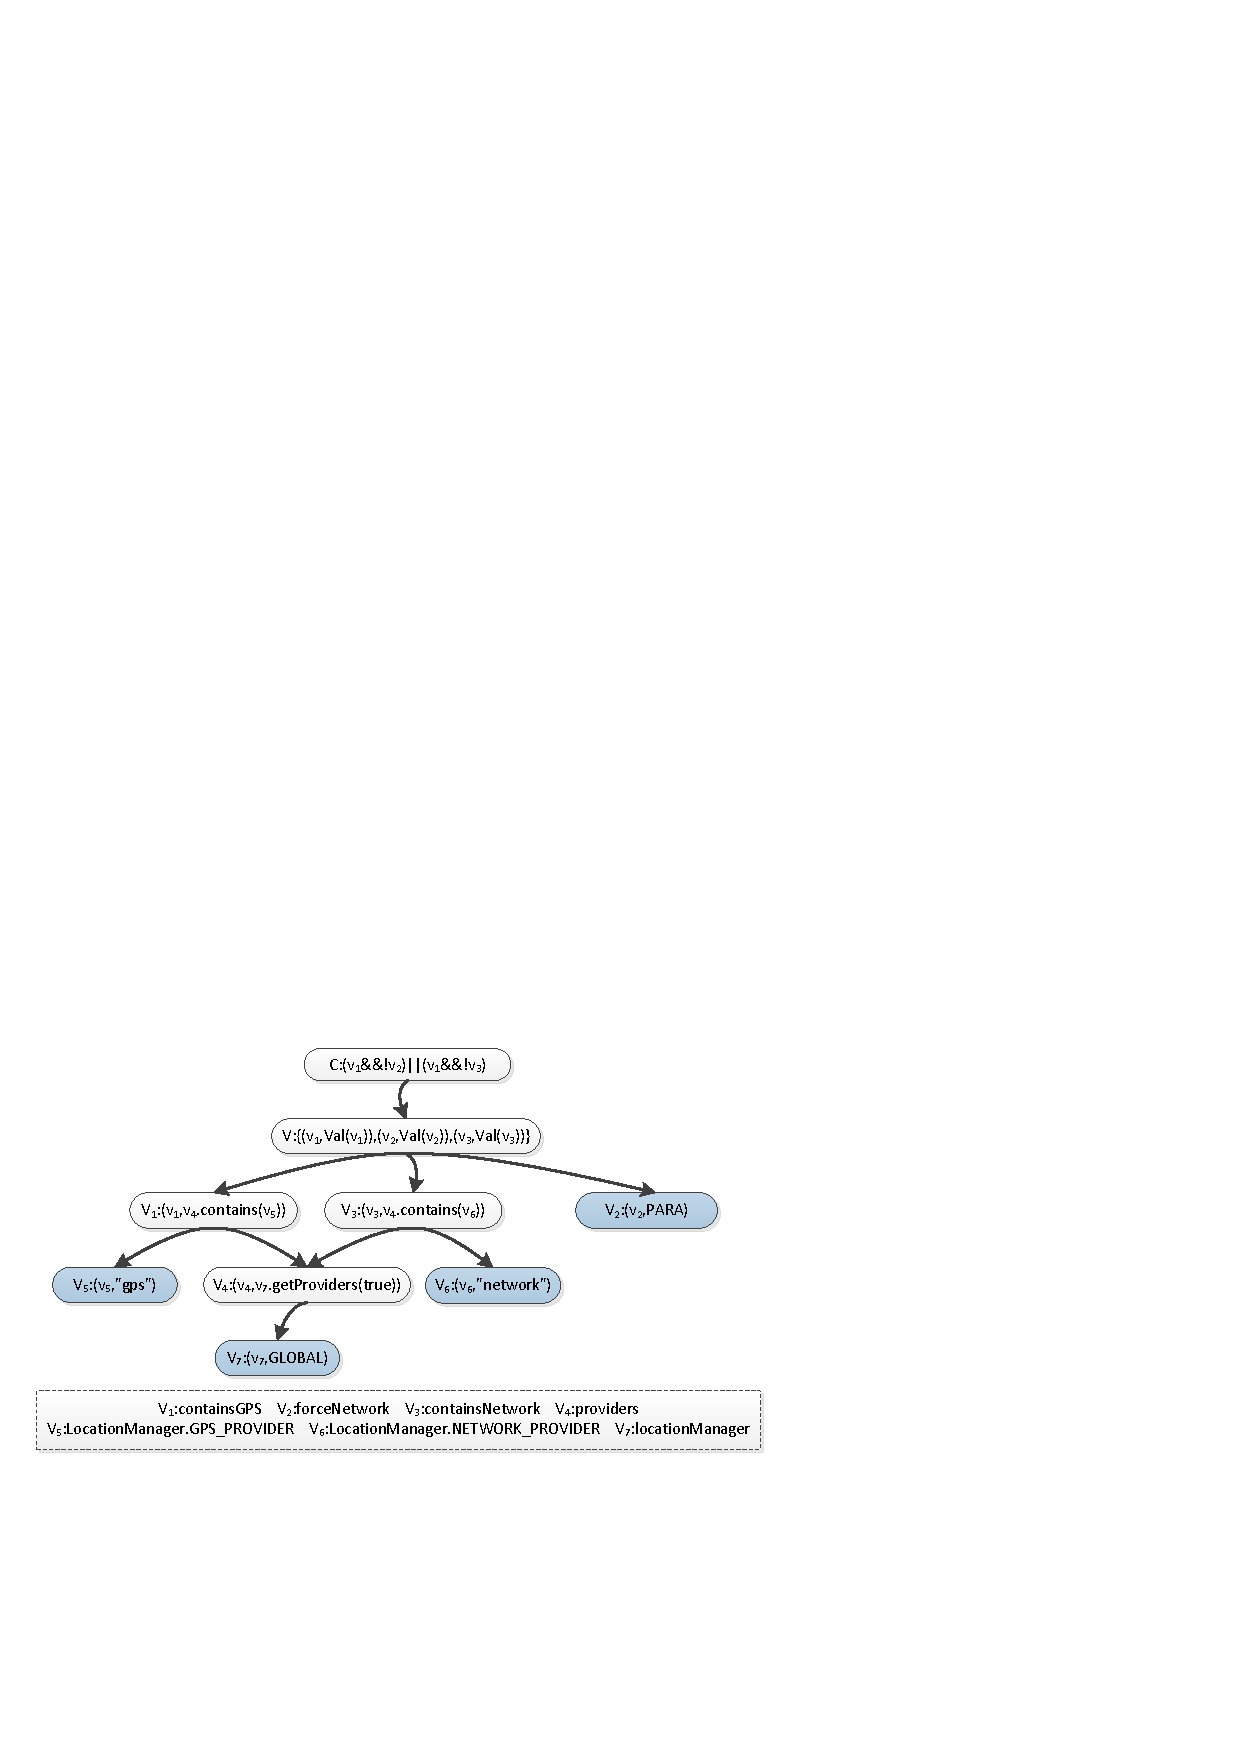
\includegraphics[width=1\linewidth]{pic/motivationCondition.pdf}  
%  \caption{Process of path-sensitive condition for motivation example.}  
% \label{fig:motConds}  
%\end{figure}

%\begin{algorithm}[!t]
%\caption{Path-sensitive Inter-component Model Construction}
%\footnotesize
%\begin{algorithmic}[1]
%\Procedure {ConsPSI} {$PII_SET$, $FRA$}
%\ForAll {$ rra \in FRA $}        
%\State $          CVList \leftarrow checkCV(fra.registerSite ) $
%\While {$\not CVList.empty$}     
%\State $                 var \leftarrow CVList.pop(0)$
%\State $                 assignSite \leftarrow backTraversal(var)$
%\State $                 pathSens \leftarrow pathSens \cup (var, assignSite )$
%\If{ $assignSite.hasNewVars$ }
%\State $                     CVList \leftarrow CVList \cup assignSite.newVars$
%\EndIf
%\EndWhile    
%\State $           fra.ivr.attr \leftarrow fra.ivr.attr \cup pathSens $
%\State $           fra.ivr.attr \leftarrow fra.ivr.attr \cup getTriggerEvent(fra.ive)$
%\EndFor
%\EndProcedure
%\end{algorithmic}
%\label{fig:alg3}
%\end{algorithm}

%If a non-lifecycle callback status is active, namely St1(c)-> {active}, its register point has already been executed, namely Rt1(c)->{executed}. And vice versa. That means the status of non-lifecycle callback is determined by the execution status of corresponding register point. Therefore, instead analyzing the target callback, we choose to check the execution condition of corresponding register point. 
%We use back-check to find the branch structure and the condition content, referenced by CC, of target register point. For the obtained CC, we abstract the variables set, referenced by V. For each variable in V, we do \textit{backTraversal} data dependency analysis. 

%We store the variable as a triple (type, name, value), which is named \texttt{condTriple}. Initially, the \textit{type} and \textit{value} are set as \texttt{null}. We only concern certain types of condition variables, which shown in Figure 3. For other unknown types, we use \texttt{u} to denote them.

%The \textit{backTraversal} checks the nearest assignment along the backward of the program. Then the \textit{type} and \textit{value} are assigned as the right-value. If the right-value is a new variable, the \textit{value} of the triple will be expanded as new triple set. The \textit{backTraversal} continues the process for right-value until reaching an end point without a empty \textit{value}.

%The analyses update the condTriple for each statement in a method until a fixed point is reached. For inter-procedural cases, the \textit{backTraversal} exploits method summary to describe the data flow information within a typical method. Methods are analyzed in reverse topological order with respect to the app system’s call graph. Thus, the entire app system can be analyzed.  

%4) Path-sensitive Model. Prior work lacks handling of path-sensitive issues. However, path-sensitive modelling improvements precision of {\color{red}both program flow and model traversing}, and further, provide assistance for related research like model checking and test case generation. Path-sensitive in modelling GPC model concerns valiables and their values that can impact the active status of succeed callbacks. 

%Although traditional IFDS \cite{} considers the interprocedural and distributive problems. It is still hard to cover the problem how and when to trigger an existing callback function. In Android framework, this problem is of particular importance causing the general existence of callbacks that directly determines a program execution direction. 

%2) In theory, a non-lifecycle callback is invoked under two conditions. One is its register-site is executed; the other is the trigger event fires. In this way, a non-lifecycle callback is possible to be invoked during running of any lifecycle callback, when satisfies the two conditions. Here we don't consider 

\subsection{Jumping Confusion}\label{jumpConfusion}
% If a lifecycle callback is not implemented in the real app, it is called hidden node. In our GPC model model, hidden node will not be represented, instead of corresponding edges. For a hidden node, all its in-edges connect all its out-edges. For example, in the \texttt{onPause} acts as a hidden node, it has one in-edge (from \texttt{onResume}) and three out-edges (to \texttt{onCreate}, \texttt{onStop} and \texttt{onResume} itself). Thus, there would be three extra edges generated by GPC model, respectively \texttt{onResume} to \texttt{onCreate},  \texttt{onResume} to \texttt{onStop} and \texttt{onResume} to itself.
In activity jumping edges $E_{j-a}$, multiple jumping invokers $subIvr\subseteq Ivr\in JA$  existing in the same activity would result in \textit{jumping confusion} (mentioned in Section \ref{problem-define}). A naive solution is to generate a direct edge connecting the invoker \textit{ivr} with invokee \textit{ive}. However, this solution ignores the related lifecycle nodes (i.e., \texttt{onActiveEnd} and \texttt{onPause}) in real sequence. Our analysis adopts a marking algorithm to address the jumping confusion. For each jumping edge $E_{j-a}$, we use a unique ID to mark the edge from its \textit{ivr} to the \textit{onActiveEnd} node, and then the same ID is used to mark the edge from \textit{onPause} node to its \textit{ive}. If two jumping actions point to the same \textit{ive}, they share the same ID. An illustration example is shown in Figure \ref{fig:motivationGPC}. The edges $\$1.onClick\rightarrow shareMyPosition.onActiveEnd$ and $shareMyPosition.onPause\rightarrow option.onCreate$ are marked as ID $1$, and other two similar edges are marked as ID $2$.

%For example, when an activity \textit{a1} jumps to another one \textit{a2}. It has to pass by the \texttt{onPause} and \texttt{onStop} callbacks, whatever callback, referenced by \textit{c1}, the jump logic is located. To this end, there should be an edge connecting the \textit{c1} and  \texttt{onPause} node. Analogously, another edge should connect the \texttt{onStop} to \textit{a2}'s \texttt{onCreate}, as shown in Figure 4. However, it is unreasonable that the path c1->onPause->onStop->a3. To address this issue, we define signed edge. 
\textit{Traversal Strategy.} 
Model traversal adopts the following strategy to avoid jumping confusion. If a traversal iterator passes an edge marked \textit{n}, then it is restricted to run along with either an unmarked edge, or an edge marked \textit{n}. After the iterator passes the jumping edge, the above restriction is removed.

%This way can effectively distinguish the callback flow in jumping logic without redundancy (without the signed edge, it has to create redundant \texttt{onPause} or \texttt{onStop} node).

%If a system-driven callback does not unregister before jumping to a new activity, then the callback is still active in the new activity states. Here we don't consider such situation.








  


%\Procedure {BellmanKalaba}{$G$, $u$, $l$, $p$}
%\ForAll {$v \in V(G)$}
%\State $l(v) \leftarrow \infty$
%\EndFor
%\State $l(u) \leftarrow 0$
%\Repeat
%\For {$i \leftarrow 1, n$}
%\State $min \leftarrow l(v_i)$
%\For {$j \leftarrow 1, n$}
%\If {$min > e(v_i, v_j) + l(v_j)$}
%\State $min \leftarrow e(v_i, v_j) + l(v_j)$
%\State $p(i) \leftarrow v_j$
%\EndIf
%\EndFor
%\State $l’(i) \leftarrow min$
%\EndFor
%\State $changed \leftarrow l \not= l’$
%\State $l \leftarrow l’$
%\Until{$\neg changed$}
%\EndProcedure
%\Statex
%\Procedure {FindPathBK}{$v$, $u$, $p$}
%\If {$v = u$}
%\State \textbf{Write} $v$
%\Else
%\State $w \leftarrow v$
%\While {$w \not= u$}
%\State \textbf{Write} $w$
%\State $w \leftarrow p(w)$
%\EndWhile
%\EndIf
%\EndProcedure


%\begin{figure}[htb]
%  \centering  
%   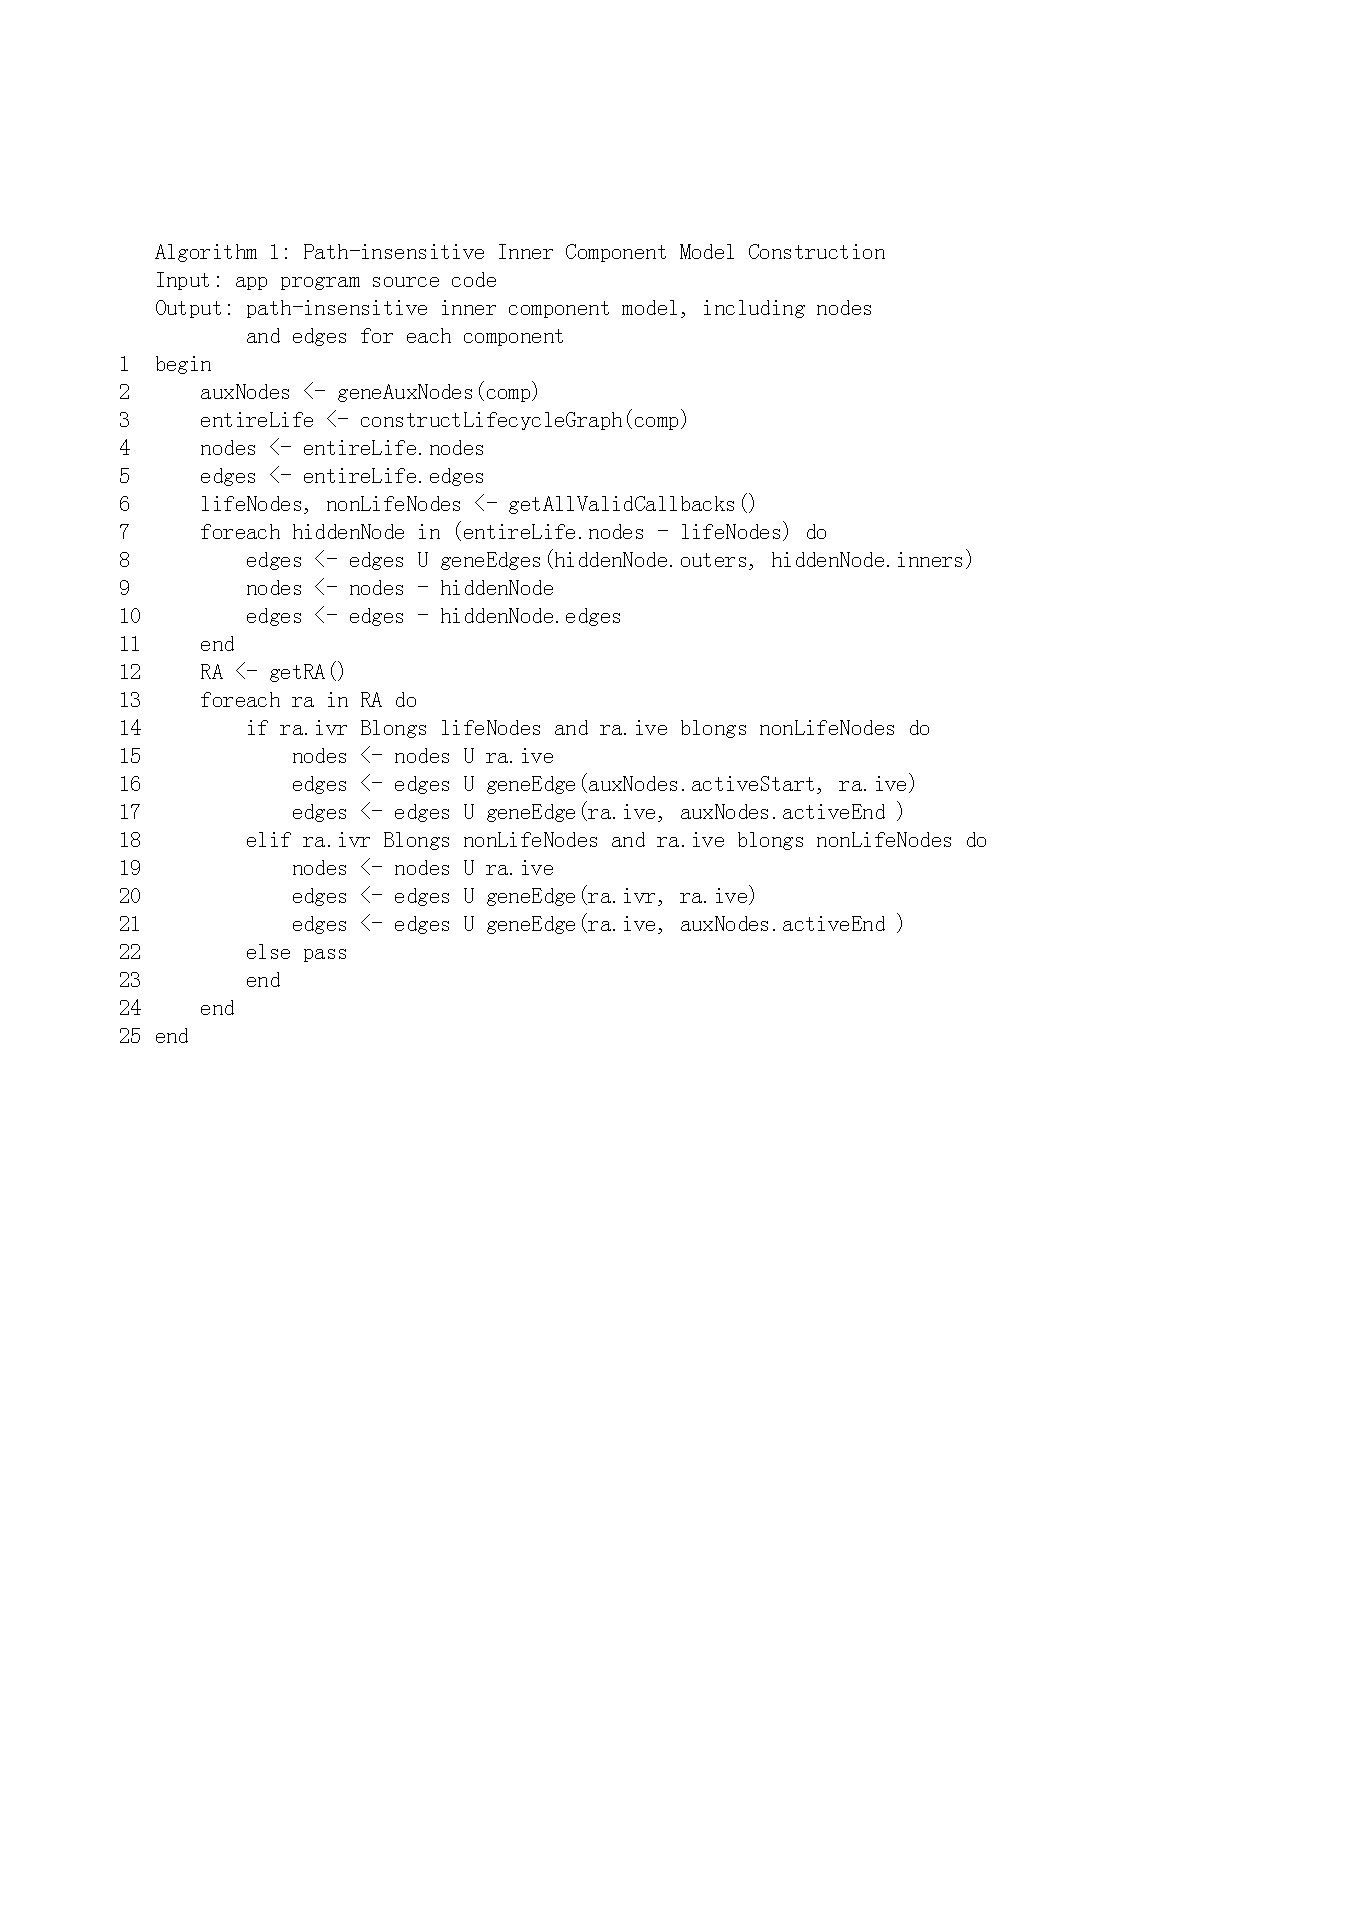
\includegraphics[width=1\linewidth]{pic/Algorithm1.pdf}   
%   %\caption{Some description about the picture}
%   \label{fig:alg1}
%\end{figure}

%\begin{figure}[htb]
%  \centering  
%   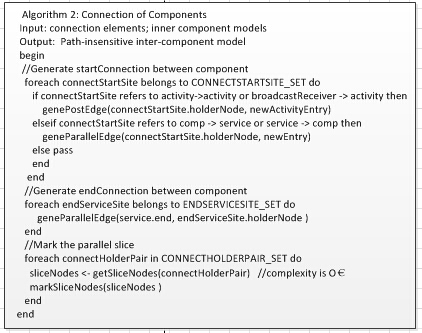
\includegraphics[width=1\linewidth]{alg2.jpg}   
%   %\caption{Some description about the picture}
%   \label{fig:alg2}
%\end{figure}

%\begin{figure}[htb]
%  \centering  
%   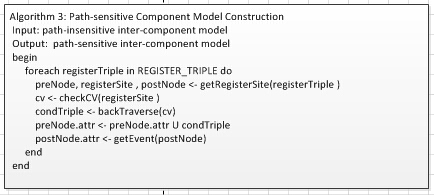
\includegraphics[width=1\linewidth]{alg3.jpg}   
%   %\caption{Some description about the picture}
%   \label{fig:alg3}
%\end{figure}

\section{Empirical Evaluation}
We implemented the method in a prototype tool -- AndroChecker, which is built based on AndroGuard~\cite{new2013androguard} framework, and consists of 4,400 lines of Python code. The input of our tool is the \textit{apk} file. The output is the set of nodes and edges, path condition set, the nodes of parallel slice and related statistical results.
%In this section, we present the empirical evaluation of our approach. First we present
We perform evaluation on 20 real-world apps downloaded from in Google Play, which are used in prior works~\cite{new2015static, new2015window}. %Considering AndroChecker is able to directly analyze the real-world apps, 
%We download these apps in Google Play, which is quite different from the prior open source version. 
Then, we study three typical cases to illustrate results of \textit{PSI} in details. 

\begin{table*}[!t]
\centering
\begin{threeparttable}[b]
\caption{Evaluation results for GPC model construction algorithms.} 
\newcommand{\tabincell}[2]{\begin{tabular}{@{}#1@{}}#2\end{tabular}}
\footnotesize

\begin{tabular}{|c|c|c|c|c|c|c|c|c|c|c|c|c|c|c|c|c|c|}
\hline 
\multirow{2}{*}{Name} &\multicolumn{3}{|c|}{Application} & \multicolumn{5}{c|}{PII} & \multicolumn{3}{c|}{CBC} & \multicolumn{3}{c|}{PSI}  &\multicolumn{2}{c|}{Time(sec)}\\
\cline{2-17}
& A & S & B &      $N_{l}$ & $E_{l}$ & $hN$ &  $N_{n}$ & $E_{r}$&     $E_{j-a}$ & $E_{j-s}$ & NSlc&   N & E & Cons&  PT & MT \\ 
\hline 
\hline 
APV & 4 & 0 & 0 &    26& 41 & 18 & 31 & 62       &9 & 0 &0 &    57 & 112 & 6     & 9 & 14\\ 
\hline 
Astrid &  57 & 16 & 27 &    304& 400 & 329 & 118 & 236      & 8 & 0 &0 &    422 & 725 & 15    & 117 & 125\\ 
\hline 
BarcodeScanner & 9 & 0 & 1 &    50& 84 & 44 & 16 & 32       &4 & 0 &0 &    66 & 120 & 3    & 18 & 38\\ 
\hline 
Beem &  13 &1 & 7 &    97& 193 & 49 & 28 & 56       &18 & 2 &- &    125 & 269 & 4    & 43 & 63\\ 

\hline 
ConnectBot & 11 & 1 & 1 &    76& 114 & 51 & 49 & 98       &9 & 1 &- &    125 & 222 & 17    & 47 & 62\\ 
\hline 
FBReader & 9 & 9 & 9 &    86& 110 & 52 & 29 & 58       &1 & 2 &- &    115 & 171 & 12    & 128 & 141\\ 
\hline 
K9 & 32 & 9 & 8 &    196& 246 & 177 & 154 & 308       &24 & 4 &- &    350 & 582 & 11    & 66 & 97\\ 
\hline 
KeePassDroid & 24 & 1 & 2 &    115& 144 & 138 & 36 & 72       &6 & 2 &4 &    151 & 224 & 16    & 11 & 18\\ 
\hline 
Mileage & 19 & 13 & 0 &    176& 209 & 98 & 79 & 158       &3 & 8 &40 &    255 & 378 & 11    & 332 & 236\\ 
\hline 
MyTracks & 7 & 1 & 1 &    42& 64 & 37 & 41 & 82       &5 & 2 &9 &    83 & 153 & 3    & 23 & 35\\ 
\hline 
NotePad & 1 & 0 & 0 &    6& 10 & 4 & 1 & 2       &0 & 0 &0 &    6 & 12 & 0    & 19 & 23\\ 
\hline 
NPR & 31 & 13 & 51 &    235& 370 & 153 & 217 & 434       &10 & 19 &- &    452 & 827 & 32    & 124 & 139\\ 
\hline 
OpenManager & 53 & 16 & 5 &    321& 596 & 272 & 272 & 544       &75 & 8 &- &    593 & 1223 & 1    & 119 & 121\\ 
\hline 
OpenSudoku & 10 & 0 & 0 &    62& 88 & 49 & 39 & 78       &14 & 0 &0 &    101 & 180 & 6    & 3 & 5\\ 
\hline 
SipDroid & 21 & 3 & 16 &    127& 203 & 106 & 48 & 96       &14 & 7 &16 &    175 & 312 & 10    & 15 & 26\\ 
\hline 
SuperGenPass & 2 & 0 & 1 &    11& 19 & 10 & 18 & 36       &1 & 0 &0 &    29 & 56 & 0    & 5 & 6\\ 
\hline 
TippyTipper & 83 & 11 & 102 &    536& 848 & 359 & 373 & 746       &362 & 127 &817 &    909 & 2083 & 58    & 251 & 376\\ 
\hline 
VLC & 24 & 11 & 11 &    189& 248 & 112 & 211 & 422       &23 & 6 &15 &    400 & 699 & 10    & 99 & 113\\ 
\hline 
VuDroid & 5 & 0 & 0 &    22& 30 & 30 & 4 & 8       &0 & 0 &0 &    26 & 38 & 0    & 1 & 2\\ 
\hline 
XBMC & 3 & 0 & 0 &    11& 15 & 19 & 0 & 0       &2 & 0 &0 &    11 & 17 & 0    & 0.1 & 0.1\\ 
\hline
\end{tabular}
%\begin{tablenotes}
    %\item [1] 
  % \end{tablenotes}
\label{tb2: experiment1}  
\end{threeparttable}
\end{table*}


% Our system is available in website.
\subsection{Construction GPC model}
Table~\ref{tb2: experiment1} shows the evaluation results for each stage of analysis. Column ``Application'' shows the component sizes, where ``A", ``S" and ``B" represent the number of activity, service and broadcast receiver, respectively. %As described in Section \ref{background}, broadcast receiver is regarded as non-lifecycle callback listener. Therefore its callbacks are added into $N_{n}$, and related inner-component edges are added into $E_{r}$.
%
Column ``PII" shows the results of the inner component model, including: lifecycle nodes $N_{l}$, lifecycle edges $E_{l}$, hidden nodes $hN$, non-lifecycle nodes $N_{n}$ and register edges $E_{r}$. %On the whole, the complexity of \textit{PII} is closely related to the component size. The number of edges are more than corresponding nodes because each node at least has a pair of incoming and outgoing, except the start and terminal nodes. Normally, the number of $E_{r}$ should be twice as many as $N_{n}$, because all the $N_{n}$ are located between \textit{onActiveStart} and \textit{onActiveEnd} with two new edges added. This relationship is based on the assumption that each non-lifecycle callbacks are invoked in the \textit{active area}, and this assumption simplifies the model complexity. Another relationship between component sizes and lifecycle nodes is reflected in the formula $N_{l} + hN = A*10 + S*6 $ or $ N_{l} + hN = A*10 + S*7$. The number of lifecycle callbacks for a component (activity and service) is fixed. For activity, the number is 10, which includes 7 regular callbacks and 3 auxiliary callbacks. For service, the number in binding mode is 7 (4 regular callbacks and 3 auxiliary callbacks), and the number in starting mode is 6 (3 regular callbacks and 3 auxiliary callbacks). However, since some callbacks are invoked along with the \texttt{onCreate} (e.g., onCreateDialog which is adopted in the motivation example), we treat them as \texttt{onCreate} lifecycle nodes. As a result, the $N_{l} + hN$ are more than $A*10 + S*7$ in some apps, e.g., \textit{APV}.
%
Column ``CBC" shows the results of the inter component connections, including: the number of inter-component edges between activities $E_{j-a}$, the number of inter-component edges involving service $E_{j-s}$ and the sum of parallel slice nodes $NSlc$. %Normally, each activity and service should be launched through other component. Therefore the number of $E_{j-a}$ and $E_{j-s}$ should be similar to \textit{A} and \textit{S} respectively. However, the $E_{j-a}$ in some apps (e.g., \textit{Astrid} and \textit{NPR}) has a large gap to the expectation in Table \ref{tb2: experiment1}. This is caused by three reasons: \textcircled{1} activities launched by other apps can not be used to generate edges. \textcircled{2} activities and services launched by implicit intents can not be recognized. \textcircled{3} context-sensitive structure can not be handled, e.g., a loop structure launches multiple services. For $NSlc$ column, "-" represents that the parallel slice can not be counted; it exists in the scenario that a service is not terminated by the activity that launches it.
%
Column ``PSI" shows the result of path-sensitive conditions. We present the total nodes $N$ and total edges $E$ in this stage. From Table \ref{tb2: experiment1}, two formulas can be observed, which are $N = N_{l} + N_{n}$ and $E = E_{l} + E_{r} + E_{j-a} + E_{j-s}$. Column ``Cons" represents the path sensitive condition number of callback flow in each app. As mentioned earlier, currently AndroChecker only supports inner-procedural conditions traversal. So the conditions residing out of the callback holder method would not be analysed. 

We omit the results of marked edges (mentioned in Section \ref{jumpConfusion}) since they are the same as $E_{j-a}$. Column ``Time" shows the time cost of our approach. It includes two parts: parsing time (\textit{PT}) and modelling time (\textit{MT}). Since AndroChecker directly handles \textit{apk} file, the process of reverse engineering consumes significant time cost. This part of work is done by AndroGuard, which is not counted. On the whole, the number of \textit{PT} and \textit{MT} are related to the components' size. 

\begin{table}[!t]
\centering
\begin{threeparttable}[b]
\caption{Example path sensitive conditions in studied cases. } 
\newcommand{\tabincell}[2]{\begin{tabular}{@{}#1@{}}#2\end{tabular}}
\footnotesize

\begin{tabular}{|c|c|c|c|}
\hline 
Name &  PSC(smali) & N & F\\
\hline 
\hline 
\multirow{6}{0.8cm}{Beem }& \multirow{2}{5.8cm}{if-eq\{SharedPreferences;$\rightarrow$getBoolean (String;Z)Z, 
String;$\rightarrow$equals(PARA;)Z\} } & \multirow{2}{*}{2}  & \multirow{2}{*}{0}\\
&&&\\
\cline{2-4}
 & \multirow{2}{5.8cm}{if-eq\{AsyncTask;$\rightarrow$getStatus()AsyncTask \$Status;,GLOBAL\}}  &\multirow{2}{*}{1} & \multirow{2}{*}{0}\\

&&&\\
 \cline{2-4}
  & \multirow{2}{5.8cm}{if-eq\{ChangeStatus;$\rightarrow$access\$1400(ChangeStatus;) Landroid/widget/Button;\}} &\multirow{2}{*}{1} & \multirow{2}{*}{1}\\
  &&&\\
\hline 
\multirow{2}{0.8cm}{My- Tracks}  &if-eq\{Utilities;$\rightarrow$isGpsOn(Context;)Z\} & 2 &1\\
\cline{2-4} 
 &if-ne\{GooglePlayServicesUtil;$\rightarrow$a(Context; I)String;\} & 1 & 0\\
\hline 
\multirow{3}{0.8cm}{Open- Sudoku}  & if-ne\{InputMethod;$\rightarrow$isInputMethodViewCreated()Z'\}  & 1&  0\\
\cline{2-4}
 & if-eq \{File;$\rightarrow$isDirectory()Z, File;$\rightarrow$isFile()Z\} &1&  1\\
\cline{2-4}
   & if-ne \{Iterator;$\rightarrow$hasNext()Z\}& 4&  0\\
\hline 
\end{tabular}
%\begin{tablenotes}
%    \item [1] 
%\end{tablenotes}
\label{tb2: experiment2}  
\end{threeparttable}
\end{table}
%
\subsection{Path Sensitive Conditions (PSC) Discussions}

We further manually study the \textit{PSC} results on three typical apps shown in Table \ref{tb2: experiment2}, where the column ``PSC" represents the simplified \textit{PSC} results; column ``N" shows the times a \textit{PSC} appears;  
%column \textit{TranToJAVA} presents the translated JAVA code from the \textit{PSC} results; 
and column ``F" shows the false positive (FP) in \textit{N}. 
%Due to the limitation of space, we combine the variable defining and using together in \textit{TranToJAVA}. E.g., for \texttt{Object c ; b==c;}, we simplified as \texttt{b==Object c;}. 

\subsubsection{Beem}
\textit{Beem} provides a full featured and easy to use XMPP client on Android. As shown in Table \ref{tb2: experiment1}, app \textit{Beem} contains four \textit{PSC}s.
% Three of them are designed to constrain unregister actions (Definition 2), and the last one is used to constrain jumping actions (Definition 2). The unregister and jumping actions include \texttt{Button.setOnClickListener}, \texttt{View.setOnCreateContextMenuListener} and \texttt{Context.bindService}. 
By manual analysis, the real conditions contains: \textcircled{1} \texttt{if ( SharedPreferences paramSharedPreferences.getBoolean("use\_auto\_awa}  \\
\texttt{y", false) \&\& "use\_auto\_away".equals(paramStrin}\\
\texttt{g) )}; \textcircled{2} \texttt{if(LoginAnim.this.mTask.getStatus()==Async}\\
\texttt{Task.Status.PENDING)}; \textcircled{3} \textit{FP}. For \textcircled{1} and \textcircled{2}, the conditions are abstracted successfully. As for \textcircled{3}, the jumping action \texttt{bindService} is directly contained by \texttt{onResume}, which indicates \textcircled{3} is an \textit{FP}. The reason is that the back traversal of AndroChecker can not correctly identify the loop structure. In details, AndroChecker treats \texttt{while()\{\} bindService;} as \texttt{while()\{bindService;\}}. Currently, in the codes generated by AndroGuard, distinguishing the two structures is intractable. This provides a direction for future improvement.

\subsubsection{MyTracks}
\textit{MyTracks} helps travellers to look for a way to keep tracking the places that they have been to. 
%Three \textit{PSC}s are detected in \textit{MyTracks}.  All the \textit{PSC}s are designed to constrain register actions. The register actions include \texttt{LocationManager.requestLocationUpdates } and \texttt{Button.setOnClickListener}. 
By manual analysis, the real \textit{PSC}s can be abstracted as  \textcircled{1} \texttt{if(Utilities.isGpsOn(getApplicationContext()))}, \textcircled{2} \textit{FP}, \textcircled{3} \texttt{if (GooglePlayServicesUtil.a(localContext,}\\
 \texttt{i).str1!=null)}. For \textcircled{1}, the real \textit{PSC} is successfully matched as shown in Table \ref{tb2: experiment2}. For \textcircled{2}, the register action is directly contained by \textit{onCreate}, and the reason of \textit{FP} is the same as in \textit{Beem}. For \textcircled{3}, the \textit{PSC} abstracted by our approach lacks the variable \textit{str1}. This is because \textit{str1} is an attribute of \textit{GooglePlayServicesUtil.a},  which can not be recognized by AndroChecker.

\subsubsection{OpenSudoku}
\textit{OpenSudoku} is an open source sudoku game. AndroChecker detects six \textit{PSC}s in \textit{OpenSudoku}.
% Five of them are designed to constrain register actions, and the last one is designed to constrain jumping actions. The register and jumping actions contain \texttt{Button.setOnClickListener} and \texttt{Context.startActivity}. 
Through manual analysis, the real \textit{PSC}s can be abstracted as \textcircled{1} \texttt{if(!(InputMethod).isInputMethodViewCreated())}, \textcircled{2} \textit{FP}, \textcircled{3} \texttt{if(!Iterator.hasNext())}.
The \textit{PSC} \textcircled{1} and \textcircled{3} are successfully detected by AndroChecker. %and they have the same semantic with the corresponding items in Table \ref{tb2: experiment2}. 
Similarly, %to \textit{MyTracks} and \textit{Beem}, 
the \textit{FP} occurs because of the loop obstacle.


%Note that the $!$ in 1) and 3) is reflected in the Table \ref{tb2: experiment2}, because it is related to the operator of byte code. 



 


%In its ten activities, seven of them contains register actions, and six of them contains jumping actions.  As shown in Table \ref{tb2: experiment1}, AndroChecker checks six valid path sensitive conditions. Four \textit{PSC}s are contained in class \texttt{IMPopupDialog}, and one condition is in class \texttt{IMControlPanelActivity}. The register actions of these five are \texttt{Button.setOnClickListener}s. The rest one is in \texttt{FileListActivity\$3}, whose register action is inter component jumping \texttt{startActivity}. Table ** shows the typical example for one of the \texttt{setOnClickListener}. The shown condition means the register action is under the condition of "if "
  

\section{Conclusion}
Prior work targeting at constructing control-flow based model in Android, provides limited benefit when applied to real systems. %Under this observation, 
We proposed GPC, a generic representation with fine-grained path information, and developed algorithms for its construction and traversal. We described our proof-of-concept builder AndroChecker and presented the evaluation results on real apps, which evidenced the efficiency of AndroChecker. %The results showed that AndroChecker can efficiently construct the expected GPC model in a fully automated way. 




\section{Acknowledgement}
This research was partially supported by a grant from the National Research 
Foundation, Prime Minister’s Office, Singapore under its National Cybersecurity 
R\&D Program (TSUNAMi project, Award No.NRF2014NCR-NCR001-21) and administered 
by the National Cybersecurity R\&D Directorate.

%\section{Related Work}
\textbf{Event-based system analysis}
One problem in event-based system such as Android is that the program execution is nondeterministic. Various existing works focus on addressing the challenges raised by such nondeterminism. \cite{new2015anomalies} proposes a static analysis approach called \textit{DEvA} to detect the event anomalies. The analysis process adopts several system representations, such as \textit{CFG}, \textit{ICFG} (inter-procedural \textit{CFG}) and \textit{PDG} (Program Dependence Graph). \cite{new2013identifying} presents \textit{Eos}, a static analysis technique that identifies message information for distributed event-based system and exploits data dependency analysis to produce \textit{MFG}(message flow graph). \cite{new2013p} provides a safe language \textit{P} for event-driven asynchronous systems and presents the interaction system via state machines. Compared with these event-based works, our work aims at constructing a generic model for better understanding of target Android app.

%cite{yang2015static} fundamentally proposes a program representation built by context-sensitive static analysis of callback methods to model the app's GUI. cite{kim2014fepma} provides an event-driven analysis manner to measure the power dissipation.  cite{chen2013contextual} centres around so-called Permission Event Graph built with static analysis and uses model checking to illegal interaction between an application and the Android event system. Again, cite{jensen2013automated} handle event-driven analysis to reach challenging source code for application testing. cite{machiry2013dynodroid} presents Dynodroid to monitor the reaction of an app upon each event either from system or user. cite{hsiao2014race}presents a race detection tool named CAFA for event-driven mobile systems. Although prior works present different insights of event-driven analysis in Android system, there are few efforts concerning the security impact raised by public event abuse. Our work fills this gap via systematic study of Android system design and statical analysis for a large scale of real-world apps. 
\textbf{Path-sensitive static Analysis}
Path-sensitive analysis (\textit{PSA}) benefits the program verification accuracy for they are able to reason about branch correlations.
\cite{new2013path3} exploits \textit{PSA} to detect remote code execution vulnerability on web application; while \cite{new2003path2} and \cite{new2005path6} use it to detect memory access errors. \cite{new2007path7} presents \textit{CHRONICLER}, an analyse tool that can infer accurate function precedence via inter-procedural \textit{PSA}. \cite{new2012path4} provides a path-sensitive static analyzer \textit{PAGAI} that computes inductive invariants on the numerical variables of the analyzed program.
Other works focus on improving path-sensitive analysis techniques. \cite{new2002path1} implements a verification tool \textit{ESP} that can engage \textit{PSA} in polynomial time. \cite{new2008path5} distinguishes observable and unobservable variables in path-sensitive program. Differing from previous works, we adopt \textit{PSA} to present a fine-grained callback invocation in produced model.

\textbf{Flow analyses and modelling for Android}
Program control/data flow analysis is widely used in areas of Android testing\cite{new2012concolic}\cite{new2013automated} and security \cite{new2014flowdroid}\cite{new2015DroidSafe}. Further, some prior works concern the impacts of ICC(inter-component communication) mechanism \cite{new2013epicc}\cite{new2015iccta}. These approaches aim at improving the precision via fine-grained flow- or context-sensitive static analysis.
Since Android contains a vast scale of SDKs(software development kit) and frameworks with complex inner mechanisms, recent works tend to abstract and construct a valid model to simplify analysis. \cite{new2015static} proposes representation \textit{CCFG} (callback control flow graph) for Android app, which is built using context-sensitive static analysis. \cite{new2015window} proposes the \textit{WTG}(window transition graph) to handle the possible \textit{GUI} window sequences, and develops algorithms for \textit{WTG} construction. \cite{new2013contextual} constructs \textit{PEG} (permission event graph) and checks malicious interaction via model checking. \cite{new2015jumping} abstracts useful control flow model in app to handle valid event orderings. Yet, these modelling efforts neither consider the impacts of flow condition, nor support fined-grained callbacks like system-driven callbacks and the callbacks from service. Our approach aims to construct a generic, path-sensitive and fine-grained callback model. 






%The exploration and exploitation of weaknesses within either Android system or apps are intensively focused by current related researchers. The study of memory side-channel analysis and exploitationcite{zhou2013identity, chen2014peeking, jana2012memento}uncovers an indirect attack way aiming to the weak architecture of Android public data exposure.
%Several recent researches focus on the vulnerabilities raised by Android advertising librariescite{soteris2016free}cite{sooel2016mob_ads}. Besides that, cite{zhang2016life} proposes data residue problem during app uninstallation. As a direct interaction channel with users, the Android UI also suffers from severity security threats, which is carefully discussed in cite{ren2015towards}cite{bianchi2015app}cite{akhawe2014clickjacking}cite{luo2012touchjacking}cite{huang2012clickjacking}cite{roesner2013securing}cite{lin2014screenmilker}. 
%Again,in the work of cite{mylonas2013smartphone}cite{xu2012taplogger}cite{miluzzo2012tapprints}, the sensor data could also be regarded as a sort of attack resources predicting some isolated private information including user input,fingerprints. In addtion, cite{armando2012dos} introduces a denial-of-service attack approach utilizing the AMS design defect. cite{xing2014upgrading} and cite{bugiel2012towards} present detailed studies about privilege escalation for malware through defects of Android os.  As to Android permission mechanism, cite{felt2011android}cite{au2012pscout}cite{zhang2013vetting}cite{fang2014permission} reveal security threats arised by the abuse of permission requests and propose corresponding migration strategy.
%In contrast to existing work, this paper represents the impact of public event defect of Android that affects a much wider range of system components and services. The attacks relying on such public event callbacks are firstly studied systematically.
%
%Android Vulnerability Detection
%As a critical security concerning on Android system, privacy data leakage incurs widely related research efforts. 
%Of all the detection works, dynamic taint tracking cite{enck2014taintdroid}cite{klieber2014android}cite{rastogi2013appsplayground}cite{poeplau2014execute} receives much eyesights for its sound accuracy.
%Another important complement for dynamic approach relies on static analysiscite{lu2012chex}cite{arzt2014flowdroid}cite{gordon2015DroidSafe}, which can effectively reduce the false negative rate. Further works concern the impacts of ICC(inter-component communication) mechanismcite{cao2015edgeminer}cite{octeau2013epicc}cite{li2015iccta}. In addition,
%cite{cox2014spandex} measures implicit leak of user password using symbolic execution. Our work is devoted to uncover the public event threats within real market app, which can be easily exploited by attackers to build a wide spectrum of new malwares. 




% An example of a floating figure using the graphicx package.
% Note that \label must occur AFTER (or within) \caption.
% For figures, \caption should occur after the \includegraphics.
% Note that IEEEtran v1.7 and later has special internal code that
% is designed to preserve the operation of \label within \caption
% even when the captionsoff option is in effect. However, because
% of issues like this, it may be the safest practice to put all your
% \label just after \caption rather than within \caption{}.
%
% Reminder: the "draftcls" or "draftclsnofoot", not "draft", class
% option should be used if it is desired that the figures are to be
% displayed while in draft mode.
%
%\begin{figure}[!t]
%\centering
%\includegraphics[width=2.5in]{myfigure}
% where an .eps filename suffix will be assumed under latex, 
% and a .pdf suffix will be assumed for pdflatex; or what has been declared
% via \DeclareGraphicsExtensions.
%\caption{Simulation Results}
%\label{fig_sim}
%\end{figure}

% Note that IEEE typically puts floats only at the top, even when this
% results in a large percentage of a column being occupied by floats.


% An example of a double column floating figure using two subfigures.
% (The subfig.sty package must be loaded for this to work.)
% The subfigure \label commands are set within each subfloat command, the
% \label for the overall figure must come after \caption.
% \hfil must be used as a separator to get equal spacing.
% The subfigure.sty package works much the same way, except \subfigure is
% used instead of \subfloat.
%
%\begin{figure*}[!t]
%\centerline{\subfloat[Case I]\includegraphics[width=2.5in]{subfigcase1}%
%\label{fig_first_case}}
%\hfil
%\subfloat[Case II]{\includegraphics[width=2.5in]{subfigcase2}%
%\label{fig_second_case}}}
%\caption{Simulation results}
%\label{fig_sim}
%\end{figure*}
%
% Note that often IEEE papers with subfigures do not employ subfigure
% captions (using the optional argument to \subfloat), but instead will
% reference/describe all of them (a), (b), etc., within the main caption.


% An example of a floating table. Note that, for IEEE style tables, the 
% \caption command should come BEFORE the table. Table text will default to
% \footnotesize as IEEE normally uses this smaller font for tables.
% The \label must come after \caption as always.
%
%\begin{table}[!t]
%% increase table row spacing, adjust to taste
%\renewcommand{\arraystretch}{1.3}
% if using array.sty, it might be a good idea to tweak the value of
% \extrarowheight as needed to properly center the text within the cells
%\caption{An Example of a Table}
%\label{table_example}
%\centering
%% Some packages, such as MDW tools, offer better commands for making tables
%% than the plain LaTeX2e tabular which is used here.
%\begin{tabular}{|c||c|}
%\hline
%One & Two\\
%\hline
%Three & Four\\
%\hline
%\end{tabular}
%\end{table}


\section{Conclusion}
Existing work targeting at constructing control-flow based model in Android provides limited benefit when applied to real system. We proposed GPC, a generic representation with fine-grained path information, and developed algorithms for its construction and traversal. We described our proof-of-concept builder AndroChecker and presented the evaluation results on real apps. The results showed that AndroChecker can efficiently construct the expected GPC model in a fully automated way. 

%In this work, we start the first exploration stage to conduct callback logic verification. Our conceptual contribution is the Callback-based Model Checking(CMC), a novel, callback logic directed approach that using model checking to automatically verify the correctness and effectiveness of target system. We devised a new static analysis procedure for generating the Callback Transition Graph(CTG) from Dalvik bytecode over components and events of entire types. To validate the proposed analysis approach, we implemented a prototype system AndroCG, which is used to construct the CTGs for over 2000 common-used real-world apps and verify corresponding logic properties. The evaluation results demonstrate the ** and ** of our approach. 
%
%Our work leads to several questions, of which one is state exploration, the other is properties need to be extended to cater more verification requirements.
%
%There are amounts of avenues of future work, and we have already started pursuing some. A logical next step would be trying to adapt CMC to verify properties relevant to device run-time feature, such as measuring of energy and memory. For example, we could collect the runtime energy consumption during each callback transition and verify whether over-consumption exists in specified callback sequences.(e.g., using CMC verify properties relevant to device run-time feature, extend model form to verify richer features)

%\section*{Acknowledgment}
%%We would like to thank our anonymous reviewer for their insightful comments.
%This research was supported in part by National Natural Science Foundation of China (No. 61402264).



% trigger a \newpage just before the given reference
% number - used to balance the columns on the last page
% adjust value as needed - may need to be readjusted if
% the document is modified later
%\IEEEtriggeratref{8}
% The "triggered" command can be changed if desired:
%\IEEEtriggercmd{\enlargethispage{-5in}}



% references section

% can use a bibliography generated by BibTeX as a .bbl file
% BibTeX documentation can be easily obtained at:
% http://www.ctan.org/tex-archive/biblio/bibtex/contrib/doc/
% The IEEEtran BibTeX style support page is at:
% http://www.michaelshell.org/tex/ieeetran/bibtex/
\bibliographystyle{IEEEtran}
%\setlength{\bibspacing}{\baselineskip}
%\bibliographystyle{abbrv}
% argument is your BibTeX string definitions and bibliography database(s)
%\bibliography{IEEEabrv,../bib/paper}
\bibliography{sigprocNew}
%
% <OR> manually copy in the resultant .bbl file
% set second argument of \begin to the number of references
% (used to reserve space for the reference number labels box)
%\begin{thebibliography}{1}
%
%\bibitem{IEEEhowto:kopka}
%H.~Kopka and P.~W. Daly, \emph{A Guide to \LaTeX}, 3rd~ed.\hskip 1em plus
%  0.5em minus 0.4em\relax Harlow, England: Addison-Wesley, 1999.
%\bibitem{Static:Yang}  
%Yang S, Yan D, Wu H, et al. Static control-flow analysis of user-driven callbacks in Android applications[C]//Proceedings of the 37th International Conference on Software Engineering-Volume 1. IEEE Press, 2015: 89-99.
%
%\end{thebibliography}
% that's all folks
\end{document}


